
% Default to the notebook output style

    


% Inherit from the specified cell style.




    
\documentclass[11pt]{article}

    
    
    \usepackage[T1]{fontenc}
    % Nicer default font (+ math font) than Computer Modern for most use cases
    \usepackage{mathpazo}

    % Basic figure setup, for now with no caption control since it's done
    % automatically by Pandoc (which extracts ![](path) syntax from Markdown).
    \usepackage{graphicx}
    % We will generate all images so they have a width \maxwidth. This means
    % that they will get their normal width if they fit onto the page, but
    % are scaled down if they would overflow the margins.
    \makeatletter
    \def\maxwidth{\ifdim\Gin@nat@width>\linewidth\linewidth
    \else\Gin@nat@width\fi}
    \makeatother
    \let\Oldincludegraphics\includegraphics
    % Set max figure width to be 80% of text width, for now hardcoded.
    \renewcommand{\includegraphics}[1]{\Oldincludegraphics[width=.8\maxwidth]{#1}}
    % Ensure that by default, figures have no caption (until we provide a
    % proper Figure object with a Caption API and a way to capture that
    % in the conversion process - todo).
    \usepackage{caption}
    \DeclareCaptionLabelFormat{nolabel}{}
    \captionsetup{labelformat=nolabel}

    \usepackage{adjustbox} % Used to constrain images to a maximum size 
    \usepackage{xcolor} % Allow colors to be defined
    \usepackage{enumerate} % Needed for markdown enumerations to work
    \usepackage{geometry} % Used to adjust the document margins
    \usepackage{amsmath} % Equations
    \usepackage{amssymb} % Equations
    \usepackage{textcomp} % defines textquotesingle
    % Hack from http://tex.stackexchange.com/a/47451/13684:
    \AtBeginDocument{%
        \def\PYZsq{\textquotesingle}% Upright quotes in Pygmentized code
    }
    \usepackage{upquote} % Upright quotes for verbatim code
    \usepackage{eurosym} % defines \euro
    \usepackage[mathletters]{ucs} % Extended unicode (utf-8) support
    \usepackage[utf8x]{inputenc} % Allow utf-8 characters in the tex document
    \usepackage{fancyvrb} % verbatim replacement that allows latex
    \usepackage{grffile} % extends the file name processing of package graphics 
                         % to support a larger range 
    % The hyperref package gives us a pdf with properly built
    % internal navigation ('pdf bookmarks' for the table of contents,
    % internal cross-reference links, web links for URLs, etc.)
    \usepackage{hyperref}
    \usepackage{longtable} % longtable support required by pandoc >1.10
    \usepackage{booktabs}  % table support for pandoc > 1.12.2
    \usepackage[inline]{enumitem} % IRkernel/repr support (it uses the enumerate* environment)
    \usepackage[normalem]{ulem} % ulem is needed to support strikethroughs (\sout)
                                % normalem makes italics be italics, not underlines
    

    
    
    % Colors for the hyperref package
    \definecolor{urlcolor}{rgb}{0,.145,.698}
    \definecolor{linkcolor}{rgb}{.71,0.21,0.01}
    \definecolor{citecolor}{rgb}{.12,.54,.11}

    % ANSI colors
    \definecolor{ansi-black}{HTML}{3E424D}
    \definecolor{ansi-black-intense}{HTML}{282C36}
    \definecolor{ansi-red}{HTML}{E75C58}
    \definecolor{ansi-red-intense}{HTML}{B22B31}
    \definecolor{ansi-green}{HTML}{00A250}
    \definecolor{ansi-green-intense}{HTML}{007427}
    \definecolor{ansi-yellow}{HTML}{DDB62B}
    \definecolor{ansi-yellow-intense}{HTML}{B27D12}
    \definecolor{ansi-blue}{HTML}{208FFB}
    \definecolor{ansi-blue-intense}{HTML}{0065CA}
    \definecolor{ansi-magenta}{HTML}{D160C4}
    \definecolor{ansi-magenta-intense}{HTML}{A03196}
    \definecolor{ansi-cyan}{HTML}{60C6C8}
    \definecolor{ansi-cyan-intense}{HTML}{258F8F}
    \definecolor{ansi-white}{HTML}{C5C1B4}
    \definecolor{ansi-white-intense}{HTML}{A1A6B2}

    % commands and environments needed by pandoc snippets
    % extracted from the output of `pandoc -s`
    \providecommand{\tightlist}{%
      \setlength{\itemsep}{0pt}\setlength{\parskip}{0pt}}
    \DefineVerbatimEnvironment{Highlighting}{Verbatim}{commandchars=\\\{\}}
    % Add ',fontsize=\small' for more characters per line
    \newenvironment{Shaded}{}{}
    \newcommand{\KeywordTok}[1]{\textcolor[rgb]{0.00,0.44,0.13}{\textbf{{#1}}}}
    \newcommand{\DataTypeTok}[1]{\textcolor[rgb]{0.56,0.13,0.00}{{#1}}}
    \newcommand{\DecValTok}[1]{\textcolor[rgb]{0.25,0.63,0.44}{{#1}}}
    \newcommand{\BaseNTok}[1]{\textcolor[rgb]{0.25,0.63,0.44}{{#1}}}
    \newcommand{\FloatTok}[1]{\textcolor[rgb]{0.25,0.63,0.44}{{#1}}}
    \newcommand{\CharTok}[1]{\textcolor[rgb]{0.25,0.44,0.63}{{#1}}}
    \newcommand{\StringTok}[1]{\textcolor[rgb]{0.25,0.44,0.63}{{#1}}}
    \newcommand{\CommentTok}[1]{\textcolor[rgb]{0.38,0.63,0.69}{\textit{{#1}}}}
    \newcommand{\OtherTok}[1]{\textcolor[rgb]{0.00,0.44,0.13}{{#1}}}
    \newcommand{\AlertTok}[1]{\textcolor[rgb]{1.00,0.00,0.00}{\textbf{{#1}}}}
    \newcommand{\FunctionTok}[1]{\textcolor[rgb]{0.02,0.16,0.49}{{#1}}}
    \newcommand{\RegionMarkerTok}[1]{{#1}}
    \newcommand{\ErrorTok}[1]{\textcolor[rgb]{1.00,0.00,0.00}{\textbf{{#1}}}}
    \newcommand{\NormalTok}[1]{{#1}}
    
    % Additional commands for more recent versions of Pandoc
    \newcommand{\ConstantTok}[1]{\textcolor[rgb]{0.53,0.00,0.00}{{#1}}}
    \newcommand{\SpecialCharTok}[1]{\textcolor[rgb]{0.25,0.44,0.63}{{#1}}}
    \newcommand{\VerbatimStringTok}[1]{\textcolor[rgb]{0.25,0.44,0.63}{{#1}}}
    \newcommand{\SpecialStringTok}[1]{\textcolor[rgb]{0.73,0.40,0.53}{{#1}}}
    \newcommand{\ImportTok}[1]{{#1}}
    \newcommand{\DocumentationTok}[1]{\textcolor[rgb]{0.73,0.13,0.13}{\textit{{#1}}}}
    \newcommand{\AnnotationTok}[1]{\textcolor[rgb]{0.38,0.63,0.69}{\textbf{\textit{{#1}}}}}
    \newcommand{\CommentVarTok}[1]{\textcolor[rgb]{0.38,0.63,0.69}{\textbf{\textit{{#1}}}}}
    \newcommand{\VariableTok}[1]{\textcolor[rgb]{0.10,0.09,0.49}{{#1}}}
    \newcommand{\ControlFlowTok}[1]{\textcolor[rgb]{0.00,0.44,0.13}{\textbf{{#1}}}}
    \newcommand{\OperatorTok}[1]{\textcolor[rgb]{0.40,0.40,0.40}{{#1}}}
    \newcommand{\BuiltInTok}[1]{{#1}}
    \newcommand{\ExtensionTok}[1]{{#1}}
    \newcommand{\PreprocessorTok}[1]{\textcolor[rgb]{0.74,0.48,0.00}{{#1}}}
    \newcommand{\AttributeTok}[1]{\textcolor[rgb]{0.49,0.56,0.16}{{#1}}}
    \newcommand{\InformationTok}[1]{\textcolor[rgb]{0.38,0.63,0.69}{\textbf{\textit{{#1}}}}}
    \newcommand{\WarningTok}[1]{\textcolor[rgb]{0.38,0.63,0.69}{\textbf{\textit{{#1}}}}}
    
    
    % Define a nice break command that doesn't care if a line doesn't already
    % exist.
    \def\br{\hspace*{\fill} \\* }
    % Math Jax compatability definitions
    \def\gt{>}
    \def\lt{<}
    % Document parameters
    \title{Advanced\_Lane\_Finding\_writeup}
    
    
    

    % Pygments definitions
    
\makeatletter
\def\PY@reset{\let\PY@it=\relax \let\PY@bf=\relax%
    \let\PY@ul=\relax \let\PY@tc=\relax%
    \let\PY@bc=\relax \let\PY@ff=\relax}
\def\PY@tok#1{\csname PY@tok@#1\endcsname}
\def\PY@toks#1+{\ifx\relax#1\empty\else%
    \PY@tok{#1}\expandafter\PY@toks\fi}
\def\PY@do#1{\PY@bc{\PY@tc{\PY@ul{%
    \PY@it{\PY@bf{\PY@ff{#1}}}}}}}
\def\PY#1#2{\PY@reset\PY@toks#1+\relax+\PY@do{#2}}

\expandafter\def\csname PY@tok@mb\endcsname{\def\PY@tc##1{\textcolor[rgb]{0.40,0.40,0.40}{##1}}}
\expandafter\def\csname PY@tok@na\endcsname{\def\PY@tc##1{\textcolor[rgb]{0.49,0.56,0.16}{##1}}}
\expandafter\def\csname PY@tok@kn\endcsname{\let\PY@bf=\textbf\def\PY@tc##1{\textcolor[rgb]{0.00,0.50,0.00}{##1}}}
\expandafter\def\csname PY@tok@kd\endcsname{\let\PY@bf=\textbf\def\PY@tc##1{\textcolor[rgb]{0.00,0.50,0.00}{##1}}}
\expandafter\def\csname PY@tok@gt\endcsname{\def\PY@tc##1{\textcolor[rgb]{0.00,0.27,0.87}{##1}}}
\expandafter\def\csname PY@tok@nb\endcsname{\def\PY@tc##1{\textcolor[rgb]{0.00,0.50,0.00}{##1}}}
\expandafter\def\csname PY@tok@nt\endcsname{\let\PY@bf=\textbf\def\PY@tc##1{\textcolor[rgb]{0.00,0.50,0.00}{##1}}}
\expandafter\def\csname PY@tok@go\endcsname{\def\PY@tc##1{\textcolor[rgb]{0.53,0.53,0.53}{##1}}}
\expandafter\def\csname PY@tok@cs\endcsname{\let\PY@it=\textit\def\PY@tc##1{\textcolor[rgb]{0.25,0.50,0.50}{##1}}}
\expandafter\def\csname PY@tok@s2\endcsname{\def\PY@tc##1{\textcolor[rgb]{0.73,0.13,0.13}{##1}}}
\expandafter\def\csname PY@tok@sa\endcsname{\def\PY@tc##1{\textcolor[rgb]{0.73,0.13,0.13}{##1}}}
\expandafter\def\csname PY@tok@sx\endcsname{\def\PY@tc##1{\textcolor[rgb]{0.00,0.50,0.00}{##1}}}
\expandafter\def\csname PY@tok@nd\endcsname{\def\PY@tc##1{\textcolor[rgb]{0.67,0.13,1.00}{##1}}}
\expandafter\def\csname PY@tok@sr\endcsname{\def\PY@tc##1{\textcolor[rgb]{0.73,0.40,0.53}{##1}}}
\expandafter\def\csname PY@tok@c1\endcsname{\let\PY@it=\textit\def\PY@tc##1{\textcolor[rgb]{0.25,0.50,0.50}{##1}}}
\expandafter\def\csname PY@tok@vg\endcsname{\def\PY@tc##1{\textcolor[rgb]{0.10,0.09,0.49}{##1}}}
\expandafter\def\csname PY@tok@cm\endcsname{\let\PY@it=\textit\def\PY@tc##1{\textcolor[rgb]{0.25,0.50,0.50}{##1}}}
\expandafter\def\csname PY@tok@sd\endcsname{\let\PY@it=\textit\def\PY@tc##1{\textcolor[rgb]{0.73,0.13,0.13}{##1}}}
\expandafter\def\csname PY@tok@dl\endcsname{\def\PY@tc##1{\textcolor[rgb]{0.73,0.13,0.13}{##1}}}
\expandafter\def\csname PY@tok@si\endcsname{\let\PY@bf=\textbf\def\PY@tc##1{\textcolor[rgb]{0.73,0.40,0.53}{##1}}}
\expandafter\def\csname PY@tok@c\endcsname{\let\PY@it=\textit\def\PY@tc##1{\textcolor[rgb]{0.25,0.50,0.50}{##1}}}
\expandafter\def\csname PY@tok@w\endcsname{\def\PY@tc##1{\textcolor[rgb]{0.73,0.73,0.73}{##1}}}
\expandafter\def\csname PY@tok@cpf\endcsname{\let\PY@it=\textit\def\PY@tc##1{\textcolor[rgb]{0.25,0.50,0.50}{##1}}}
\expandafter\def\csname PY@tok@sb\endcsname{\def\PY@tc##1{\textcolor[rgb]{0.73,0.13,0.13}{##1}}}
\expandafter\def\csname PY@tok@gh\endcsname{\let\PY@bf=\textbf\def\PY@tc##1{\textcolor[rgb]{0.00,0.00,0.50}{##1}}}
\expandafter\def\csname PY@tok@mh\endcsname{\def\PY@tc##1{\textcolor[rgb]{0.40,0.40,0.40}{##1}}}
\expandafter\def\csname PY@tok@ne\endcsname{\let\PY@bf=\textbf\def\PY@tc##1{\textcolor[rgb]{0.82,0.25,0.23}{##1}}}
\expandafter\def\csname PY@tok@k\endcsname{\let\PY@bf=\textbf\def\PY@tc##1{\textcolor[rgb]{0.00,0.50,0.00}{##1}}}
\expandafter\def\csname PY@tok@vm\endcsname{\def\PY@tc##1{\textcolor[rgb]{0.10,0.09,0.49}{##1}}}
\expandafter\def\csname PY@tok@ch\endcsname{\let\PY@it=\textit\def\PY@tc##1{\textcolor[rgb]{0.25,0.50,0.50}{##1}}}
\expandafter\def\csname PY@tok@mo\endcsname{\def\PY@tc##1{\textcolor[rgb]{0.40,0.40,0.40}{##1}}}
\expandafter\def\csname PY@tok@vi\endcsname{\def\PY@tc##1{\textcolor[rgb]{0.10,0.09,0.49}{##1}}}
\expandafter\def\csname PY@tok@mi\endcsname{\def\PY@tc##1{\textcolor[rgb]{0.40,0.40,0.40}{##1}}}
\expandafter\def\csname PY@tok@kp\endcsname{\def\PY@tc##1{\textcolor[rgb]{0.00,0.50,0.00}{##1}}}
\expandafter\def\csname PY@tok@o\endcsname{\def\PY@tc##1{\textcolor[rgb]{0.40,0.40,0.40}{##1}}}
\expandafter\def\csname PY@tok@gi\endcsname{\def\PY@tc##1{\textcolor[rgb]{0.00,0.63,0.00}{##1}}}
\expandafter\def\csname PY@tok@nl\endcsname{\def\PY@tc##1{\textcolor[rgb]{0.63,0.63,0.00}{##1}}}
\expandafter\def\csname PY@tok@il\endcsname{\def\PY@tc##1{\textcolor[rgb]{0.40,0.40,0.40}{##1}}}
\expandafter\def\csname PY@tok@gd\endcsname{\def\PY@tc##1{\textcolor[rgb]{0.63,0.00,0.00}{##1}}}
\expandafter\def\csname PY@tok@sh\endcsname{\def\PY@tc##1{\textcolor[rgb]{0.73,0.13,0.13}{##1}}}
\expandafter\def\csname PY@tok@no\endcsname{\def\PY@tc##1{\textcolor[rgb]{0.53,0.00,0.00}{##1}}}
\expandafter\def\csname PY@tok@kc\endcsname{\let\PY@bf=\textbf\def\PY@tc##1{\textcolor[rgb]{0.00,0.50,0.00}{##1}}}
\expandafter\def\csname PY@tok@mf\endcsname{\def\PY@tc##1{\textcolor[rgb]{0.40,0.40,0.40}{##1}}}
\expandafter\def\csname PY@tok@ow\endcsname{\let\PY@bf=\textbf\def\PY@tc##1{\textcolor[rgb]{0.67,0.13,1.00}{##1}}}
\expandafter\def\csname PY@tok@nf\endcsname{\def\PY@tc##1{\textcolor[rgb]{0.00,0.00,1.00}{##1}}}
\expandafter\def\csname PY@tok@s1\endcsname{\def\PY@tc##1{\textcolor[rgb]{0.73,0.13,0.13}{##1}}}
\expandafter\def\csname PY@tok@nv\endcsname{\def\PY@tc##1{\textcolor[rgb]{0.10,0.09,0.49}{##1}}}
\expandafter\def\csname PY@tok@nc\endcsname{\let\PY@bf=\textbf\def\PY@tc##1{\textcolor[rgb]{0.00,0.00,1.00}{##1}}}
\expandafter\def\csname PY@tok@kt\endcsname{\def\PY@tc##1{\textcolor[rgb]{0.69,0.00,0.25}{##1}}}
\expandafter\def\csname PY@tok@fm\endcsname{\def\PY@tc##1{\textcolor[rgb]{0.00,0.00,1.00}{##1}}}
\expandafter\def\csname PY@tok@kr\endcsname{\let\PY@bf=\textbf\def\PY@tc##1{\textcolor[rgb]{0.00,0.50,0.00}{##1}}}
\expandafter\def\csname PY@tok@gu\endcsname{\let\PY@bf=\textbf\def\PY@tc##1{\textcolor[rgb]{0.50,0.00,0.50}{##1}}}
\expandafter\def\csname PY@tok@bp\endcsname{\def\PY@tc##1{\textcolor[rgb]{0.00,0.50,0.00}{##1}}}
\expandafter\def\csname PY@tok@gs\endcsname{\let\PY@bf=\textbf}
\expandafter\def\csname PY@tok@gr\endcsname{\def\PY@tc##1{\textcolor[rgb]{1.00,0.00,0.00}{##1}}}
\expandafter\def\csname PY@tok@sc\endcsname{\def\PY@tc##1{\textcolor[rgb]{0.73,0.13,0.13}{##1}}}
\expandafter\def\csname PY@tok@vc\endcsname{\def\PY@tc##1{\textcolor[rgb]{0.10,0.09,0.49}{##1}}}
\expandafter\def\csname PY@tok@gp\endcsname{\let\PY@bf=\textbf\def\PY@tc##1{\textcolor[rgb]{0.00,0.00,0.50}{##1}}}
\expandafter\def\csname PY@tok@ss\endcsname{\def\PY@tc##1{\textcolor[rgb]{0.10,0.09,0.49}{##1}}}
\expandafter\def\csname PY@tok@ge\endcsname{\let\PY@it=\textit}
\expandafter\def\csname PY@tok@err\endcsname{\def\PY@bc##1{\setlength{\fboxsep}{0pt}\fcolorbox[rgb]{1.00,0.00,0.00}{1,1,1}{\strut ##1}}}
\expandafter\def\csname PY@tok@s\endcsname{\def\PY@tc##1{\textcolor[rgb]{0.73,0.13,0.13}{##1}}}
\expandafter\def\csname PY@tok@nn\endcsname{\let\PY@bf=\textbf\def\PY@tc##1{\textcolor[rgb]{0.00,0.00,1.00}{##1}}}
\expandafter\def\csname PY@tok@se\endcsname{\let\PY@bf=\textbf\def\PY@tc##1{\textcolor[rgb]{0.73,0.40,0.13}{##1}}}
\expandafter\def\csname PY@tok@ni\endcsname{\let\PY@bf=\textbf\def\PY@tc##1{\textcolor[rgb]{0.60,0.60,0.60}{##1}}}
\expandafter\def\csname PY@tok@m\endcsname{\def\PY@tc##1{\textcolor[rgb]{0.40,0.40,0.40}{##1}}}
\expandafter\def\csname PY@tok@cp\endcsname{\def\PY@tc##1{\textcolor[rgb]{0.74,0.48,0.00}{##1}}}

\def\PYZbs{\char`\\}
\def\PYZus{\char`\_}
\def\PYZob{\char`\{}
\def\PYZcb{\char`\}}
\def\PYZca{\char`\^}
\def\PYZam{\char`\&}
\def\PYZlt{\char`\<}
\def\PYZgt{\char`\>}
\def\PYZsh{\char`\#}
\def\PYZpc{\char`\%}
\def\PYZdl{\char`\$}
\def\PYZhy{\char`\-}
\def\PYZsq{\char`\'}
\def\PYZdq{\char`\"}
\def\PYZti{\char`\~}
% for compatibility with earlier versions
\def\PYZat{@}
\def\PYZlb{[}
\def\PYZrb{]}
\makeatother


    % Exact colors from NB
    \definecolor{incolor}{rgb}{0.0, 0.0, 0.5}
    \definecolor{outcolor}{rgb}{0.545, 0.0, 0.0}



    
    % Prevent overflowing lines due to hard-to-break entities
    \sloppy 
    % Setup hyperref package
    \hypersetup{
      breaklinks=true,  % so long urls are correctly broken across lines
      colorlinks=true,
      urlcolor=urlcolor,
      linkcolor=linkcolor,
      citecolor=citecolor,
      }
    % Slightly bigger margins than the latex defaults
    
    \geometry{verbose,tmargin=1in,bmargin=1in,lmargin=1in,rmargin=1in}
    
    

    \begin{document}
    
    
    \maketitle
    
    

    
    \hypertarget{self-driving-car-engineer-nanodegree-writeup}{%
\section{Self-Driving Car Engineer Nanodegree
Writeup}\label{self-driving-car-engineer-nanodegree-writeup}}

\begin{center}\rule{0.5\linewidth}{\linethickness}\end{center}

\hypertarget{project-2-advanced-lane-finding}{%
\subsection{\texorpdfstring{Project 2: \textbf{Advanced Lane
Finding}}{Project 2: Advanced Lane Finding}}\label{project-2-advanced-lane-finding}}

\hypertarget{written-by-philip-renn}{%
\paragraph{\texorpdfstring{\textbf{Written by: Philip
Renn}}{Written by: Philip Renn}}\label{written-by-philip-renn}}

\begin{center}\rule{0.5\linewidth}{\linethickness}\end{center}

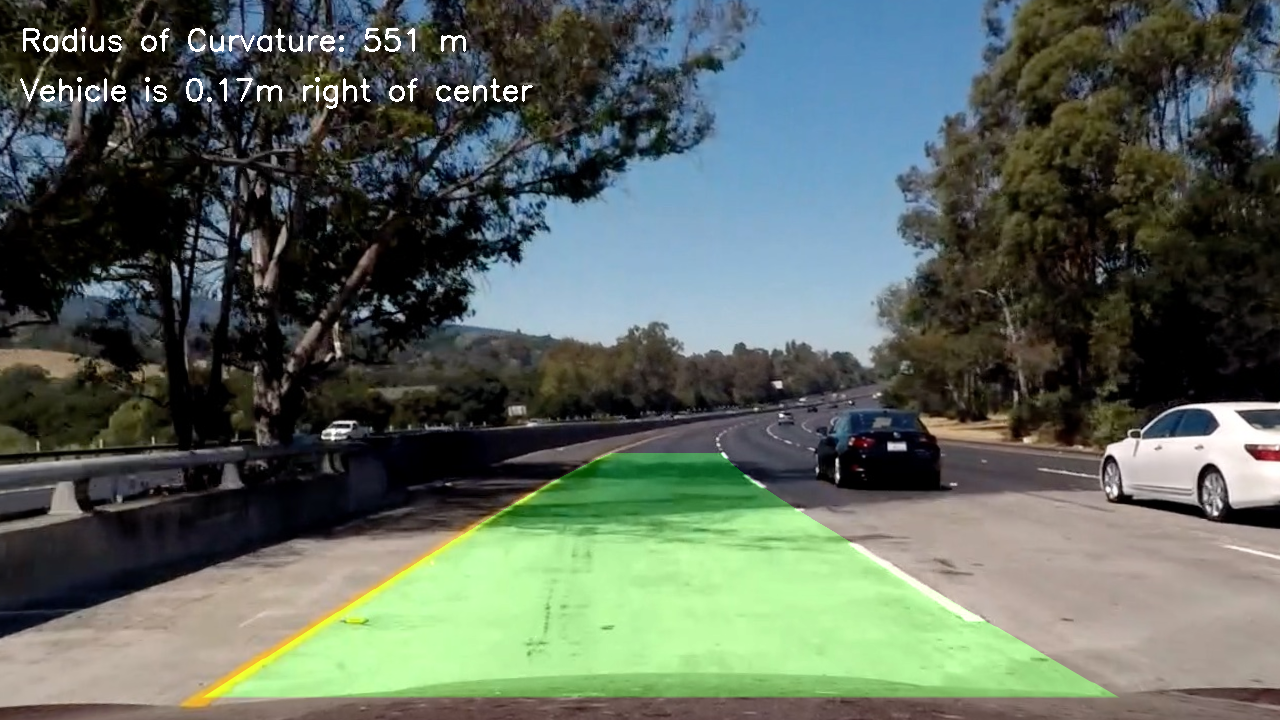
\includegraphics{./output_images/writeup_images/result.png} ***

    \hypertarget{preliminary-goal}{%
\subsection{Preliminary Goal}\label{preliminary-goal}}

\begin{verbatim}
Calibrate a 2D camera using chessboard calibration images to a aquire a conversion matrix and distortion coefficients.   
\end{verbatim}

\hypertarget{primary-goal}{%
\subsection{Primary Goal}\label{primary-goal}}

\begin{verbatim}
Write a sofetware pipeline to identiify the lane boundaries from raw images from a video.
\end{verbatim}

\hypertarget{steps}{%
\subsubsection{Steps:}\label{steps}}

\begin{itemize}
\tightlist
\item
  Apply a distortion correction to raw images.
\item
  Use color transforms, gradients, etc., to create a thresholded binary
  image.
\item
  Apply a perspective transform to rectify binary image (``birds-eye
  view'').
\item
  Detect lane pixels and fit to find the lane boundary.
\item
  Determine the curvature of the lane and vehicle position with respect
  to center.
\item
  Warp the detected lane boundaries back onto the original image.
\item
  Output visual display of the lane boundaries and numerical estimation
  of lane curvature and vehicle position.
\end{itemize}

    \hypertarget{readme}{%
\subsection{README}\label{readme}}

\begin{center}\rule{0.5\linewidth}{\linethickness}\end{center}

\hypertarget{dependencies}{%
\subsubsection{Dependencies}\label{dependencies}}

\begin{center}\rule{0.5\linewidth}{\linethickness}\end{center}

\begin{itemize}
\tightlist
\item
  Anaconda Prompt
\item
  Python 3
\item
  Matplotlib
\item
  Numpy
\item
  OpenCV
\item
  Math
\item
  Glob
\item
  Pickle
\item
  Moviepy
\item
  IPython
\item
  Collections
\item
  Jupyter Notebook
\end{itemize}

\hypertarget{files}{%
\subsubsection{Files}\label{files}}

\begin{center}\rule{0.5\linewidth}{\linethickness}\end{center}

\begin{itemize}
\item
  \texttt{./camera\_cal/} \textbar{} images used for calibrating the
  camera
\item
  \texttt{./test\_images/} \textbar{} images to test pipeline
\item
  \texttt{./output\_images/} \textbar{} processed test images of each
  step of pipeline
\item
  \texttt{./Advanced\_Lane\_Finding.ipynb} \textbar{} main code for
  processing images and video
\item
  \texttt{./project\_video\_output.mp4} \textbar{} video of processed
  ``project\_veideo.mp4''
\item
  \texttt{./camera\_calibration.ipynb} \textbar{} code to calibrate
  camera using images in ./camera\_cal/
\item
  \texttt{./calibration\_data.p} \textbar{} file containing matrix and
  distortion coeficients
\end{itemize}

\hypertarget{how-to-run-advanced_lane_finding.ipynb-using-jupyter-notebook}{%
\subsection{\texorpdfstring{How to run
\texttt{Advanced\_Lane\_Finding.ipynb} using jupyter
notebook}{How to run Advanced\_Lane\_Finding.ipynb using jupyter notebook}}\label{how-to-run-advanced_lane_finding.ipynb-using-jupyter-notebook}}

\begin{center}\rule{0.5\linewidth}{\linethickness}\end{center}

\begin{enumerate}
\def\labelenumi{\arabic{enumi}.}
\item
  Get repository from github
\item
  Open an Anaconda Prompt
\item
  cd into the directory containing the Advanced\_Lane\_Finding.ipynb
  file
\item
  Enter the command: jupyter notebook P1.ipynb
\item ~
  \hypertarget{click-on-the-kernel-tab-restart-run-all}{%
  \subsection{Click on the ``Kernel'' tab \textgreater{}\textgreater{}
  ``Restart \& Run
  All''}\label{click-on-the-kernel-tab-restart-run-all}}
\end{enumerate}

    \hypertarget{rubric-points}{%
\subsection{Rubric Points}\label{rubric-points}}

\begin{center}\rule{0.5\linewidth}{\linethickness}\end{center}

\hypertarget{camera-calibration}{%
\subsection{Camera Calibration}\label{camera-calibration}}

\hypertarget{have-the-camera-matrix-and-distortion-coefficients-been-computed-correctly-and-checked-on-the-calibration-test-image}{%
\subsubsection{1. Have the camera matrix and distortion coefficients
been computed correctly and checked on the calibration test
image?}\label{have-the-camera-matrix-and-distortion-coefficients-been-computed-correctly-and-checked-on-the-calibration-test-image}}

The code for calibrating the camera is in the file
\texttt{camera\_calibration.ipynb}.

First, I read in all calibration images and prepared \texttt{objp} to
store the object points (x,y,z) with a size to store coordinates in the
wolrd, assuming z=0. This matrix is appended to \texttt{objpoints} for
each detected image. Then, I detected the \texttt{corners} of the
chessboard and appended these points to \texttt{imgpoints} for each
detected chessboard.

I then use \texttt{objpoints} and \texttt{imgpoints} to calibrate the
camera using \texttt{cv2.calibrateCamera()} function, which will return
\texttt{mtx} and \texttt{dist} which are the calibration matrix and
distortion coefficients, respectively. The results of \texttt{mtx} and
\texttt{dist} were exported to the file \texttt{calibration\_data.p}.
These are the variables that will be used to undistort the raw images
from the video using \texttt{cv2.undistort()}. Below is an output of the
calibration process:

\begin{center}\rule{0.5\linewidth}{\linethickness}\end{center}

\begin{figure}
\centering
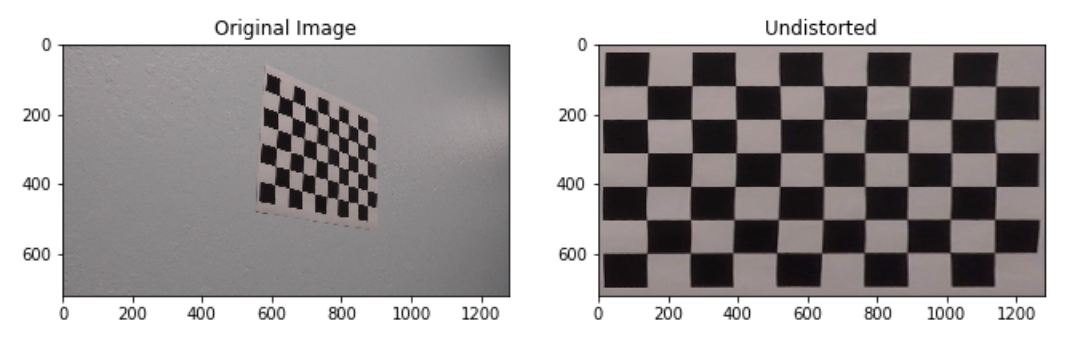
\includegraphics{./output_images/writeup_images/cal_example.png}
\caption{alt text}
\end{figure}

\begin{center}\rule{0.5\linewidth}{\linethickness}\end{center}

    \hypertarget{pipeline-single-images}{%
\subsection{Pipeline (single images)}\label{pipeline-single-images}}

\hypertarget{has-the-distortion-correction-been-correctly-applied-to-each-image}{%
\subsubsection{1. Has the distortion correction been correctly applied
to each
image?}\label{has-the-distortion-correction-been-correctly-applied-to-each-image}}

Below is an example of the distortion correction step. I imported the
\texttt{mtx} and \texttt{dist} data from the
\texttt{calibration\_data.p} file that was created in the camera
calibration step. I used these values as arguments in the
\texttt{cv2.undistort()} function which returned the undistorted image.
The unditort process corrects for the distortion caused by the camera
lens. A rounded camera lens captures more light at the edges of the
image which causes objects to appear more or less curved than they
actually are in the real world. This can be observed in the image below.
Notice the difference in position of the white car from the original
image and the undistorted image. In the orginal image the entire rear
end of the white car is visible whereas the undistorted image show less
of the rear because it was close to the edge of the frame which is
generally where the ``curved'' effect can be observed.

\begin{center}\rule{0.5\linewidth}{\linethickness}\end{center}

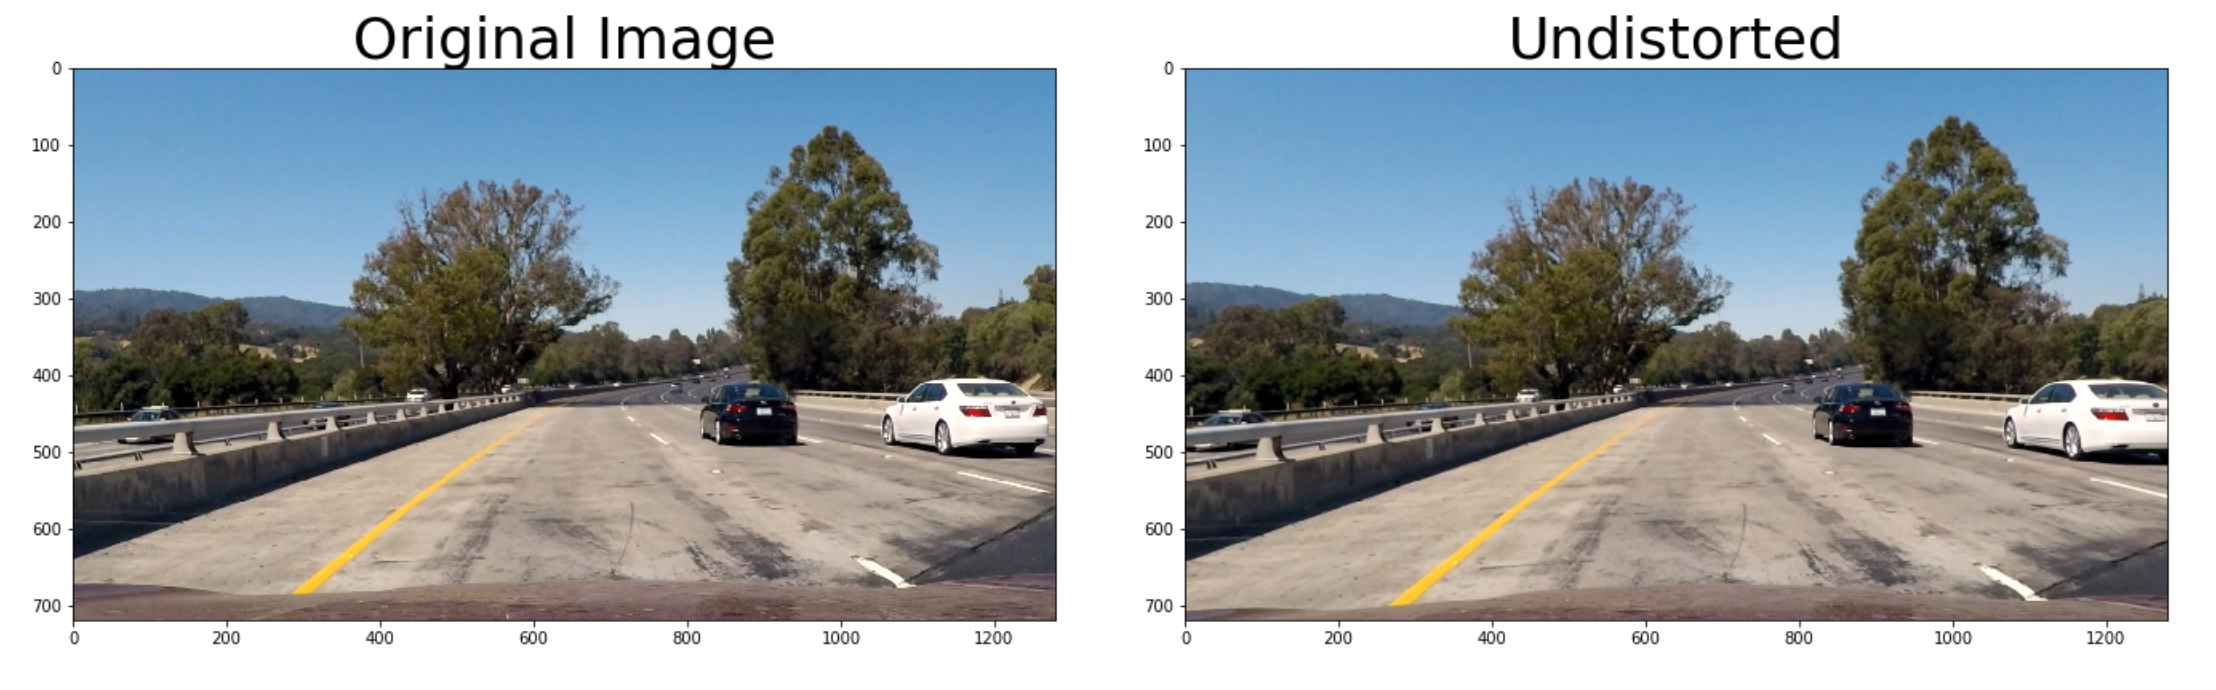
\includegraphics{./output_images/writeup_images/test1_undist.png} ***

    \hypertarget{has-a-perspective-transform-been-applied-to-rectify-the-image}{%
\subsubsection{2. Has a perspective transform been applied to rectify
the
image?}\label{has-a-perspective-transform-been-applied-to-rectify-the-image}}

Next, I applied the perspective transform using \texttt{M} to transform
the selected region \texttt{src}, determined by the initialized points,
to the destination \texttt{dst} region. This perspective transformation
returns a ``birds-eye'' view.

\begin{Shaded}
\begin{Highlighting}[]
\CommentTok{#### Perspective Transform Variables ####}
\CommentTok{# Set offset for destination points}
\NormalTok{offsetx }\OperatorTok{=} \DecValTok{400}
\CommentTok{# Defining trapezoid points for src image }
\NormalTok{imshape }\OperatorTok{=}\NormalTok{ (}\DecValTok{720}\NormalTok{, }\DecValTok{1280}\NormalTok{)}
\NormalTok{left_bottom_p }\OperatorTok{=}\NormalTok{ [}\DecValTok{217}\NormalTok{, }\DecValTok{705}\NormalTok{]}
\NormalTok{left_top_p }\OperatorTok{=}\NormalTok{ [}\DecValTok{588}\NormalTok{, }\DecValTok{453}\NormalTok{]}
\NormalTok{right_top_p }\OperatorTok{=}\NormalTok{ [}\DecValTok{694}\NormalTok{, }\DecValTok{453}\NormalTok{]}
\NormalTok{right_bottom_p }\OperatorTok{=}\NormalTok{ [}\DecValTok{1100}\NormalTok{, }\DecValTok{705}\NormalTok{]}
\CommentTok{# Set src and dst points and get matrix (and inverse) to warp perspective}
\CommentTok{# Define 4 source points src = np.float32([[,],[,],[,],[,]])}
\NormalTok{src }\OperatorTok{=}\NormalTok{ np.float32([[left_bottom_p, left_top_p, right_top_p, right_bottom_p]], dtype}\OperatorTok{=}\NormalTok{np.int32)}
\CommentTok{# Define 4 destination points dst = np.float32([[,],[,],[,],[,]])}
\NormalTok{dst }\OperatorTok{=}\NormalTok{ np.float32([[offsetx, imshape[}\DecValTok{0}\NormalTok{]],[offsetx, }\DecValTok{0}\NormalTok{],[imshape[}\DecValTok{1}\NormalTok{]}\OperatorTok{-}\NormalTok{offsetx, }\DecValTok{0}\NormalTok{],[imshape[}\DecValTok{1}\NormalTok{]}\OperatorTok{-}\NormalTok{offsetx, imshape[}\DecValTok{0}\NormalTok{]]])}
\CommentTok{# Use cv2.getPerspectiveTransform() to get M, the transform matrix, and its inverse, Minv}
\NormalTok{M }\OperatorTok{=}\NormalTok{ cv2.getPerspectiveTransform(src, dst)}
\NormalTok{Minv }\OperatorTok{=}\NormalTok{ cv2.getPerspectiveTransform(dst, src)}
\end{Highlighting}
\end{Shaded}

It is important to note that the lines should appear parallel in the
transformed image since the lines appear straight in the undistorted
image. The red lines represent the region specified by the source,
\texttt{src}, and destination, \texttt{dst}, points. An example output
of this step is shown below:

\begin{center}\rule{0.5\linewidth}{\linethickness}\end{center}

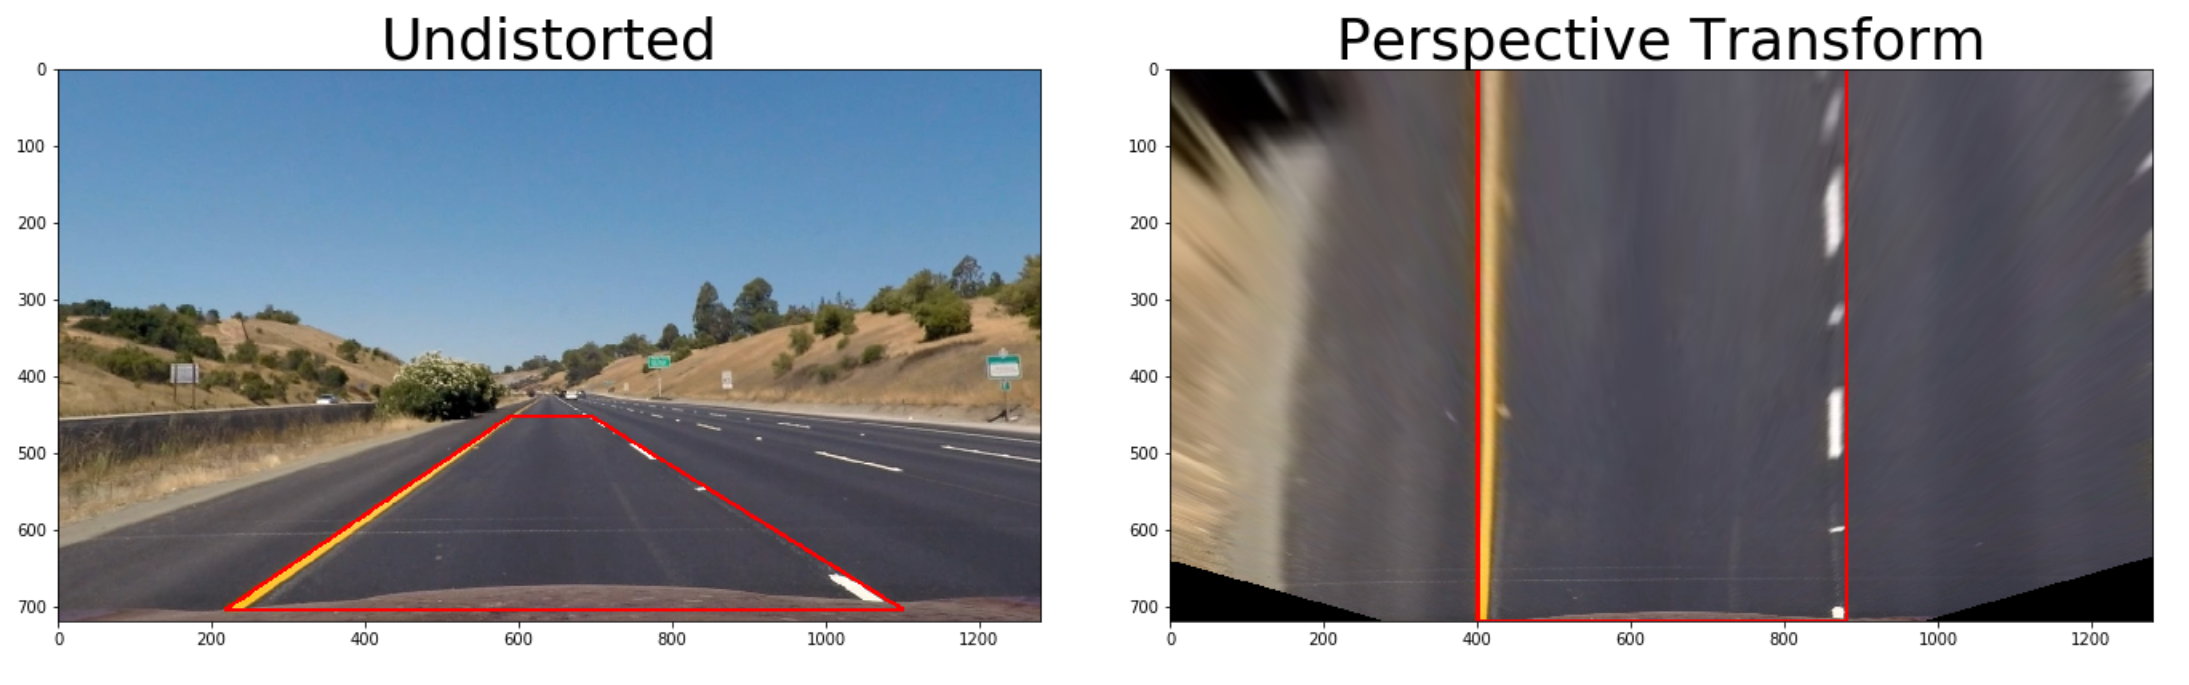
\includegraphics{./output_images/writeup_images/straight_lines1_birdseye.png}
***

    \hypertarget{has-a-binary-image-been-created-using-color-transforms-gradients-or-other-methods}{%
\subsubsection{3. Has a binary image been created using color
transforms, gradients or other
methods?}\label{has-a-binary-image-been-created-using-color-transforms-gradients-or-other-methods}}

I created a binary image as a result of a combination of thresholding
layers from difference color spaces. To do this, I transformed the BGR
image to the HLS color space and thresholded each layer H,L,S. I also
thresholded the red layer of the BGR image to detect the white lines as
white is represented best in the red layer values. I used
\href{http://colorizer.org/}{colorizer} to tune the threshold values.

The code for the \texttt{color\_select()} function below:

\begin{Shaded}
\begin{Highlighting}[]
\KeywordTok{def}\NormalTok{ color_mask(img, img_hls):}
    \CommentTok{"""}
\CommentTok{    Applies a color selection mask to find yellow & white lane line pixel values.}
\CommentTok{    Converts input image to HLS color space and thresholds each layer and performs}
\CommentTok{    bitwise operations with the Red layer from BGR image.}
\CommentTok{    }
\CommentTok{    Returns a color-masked binary image.}
\CommentTok{    """}
    \CommentTok{# Grab R layer of BGR image and H,L,S layers from HLS image}
\NormalTok{    R }\OperatorTok{=}\NormalTok{ img[:,:,}\DecValTok{2}\NormalTok{]}
\NormalTok{    H }\OperatorTok{=}\NormalTok{ img_hls[:,:,}\DecValTok{0}\NormalTok{]}
\NormalTok{    L }\OperatorTok{=}\NormalTok{ img_hls[:,:,}\DecValTok{1}\NormalTok{]}
\NormalTok{    S }\OperatorTok{=}\NormalTok{ img_hls[:,:,}\DecValTok{2}\NormalTok{]}
    
    \CommentTok{# Applying color thresholds using color space thresholds for R, H, L, S layers}
\NormalTok{    R_binary }\OperatorTok{=}\NormalTok{ np.zeros_like(R)}
\NormalTok{    R_binary[(R }\OperatorTok{>=}\NormalTok{ R_thresh[}\DecValTok{0}\NormalTok{]) }\OperatorTok{&}\NormalTok{ (L }\OperatorTok{>=} \DecValTok{150}\NormalTok{)] }\OperatorTok{=} \DecValTok{1}
\NormalTok{    H_binary }\OperatorTok{=}\NormalTok{ np.zeros_like(H)}
\NormalTok{    H_binary[(H }\OperatorTok{>=}\NormalTok{ H_thresh[}\DecValTok{0}\NormalTok{]) }\OperatorTok{&}\NormalTok{ (H }\OperatorTok{<=}\NormalTok{ H_thresh[}\DecValTok{1}\NormalTok{])] }\OperatorTok{=} \DecValTok{1}
\NormalTok{    L_binary }\OperatorTok{=}\NormalTok{ np.zeros_like(L)}
\NormalTok{    L_binary[(L }\OperatorTok{>=}\NormalTok{ L_thresh[}\DecValTok{0}\NormalTok{]) }\OperatorTok{&}\NormalTok{ (L }\OperatorTok{<=}\NormalTok{ L_thresh[}\DecValTok{1}\NormalTok{])] }\OperatorTok{=} \DecValTok{1}
\NormalTok{    S_binary }\OperatorTok{=}\NormalTok{ np.zeros_like(S)}
\NormalTok{    S_binary[(S }\OperatorTok{>=}\NormalTok{ S_thresh[}\DecValTok{0}\NormalTok{]) }\OperatorTok{&}\NormalTok{ (S }\OperatorTok{<=}\NormalTok{ S_thresh[}\DecValTok{1}\NormalTok{])] }\OperatorTok{=} \DecValTok{1}
    
    \CommentTok{# Combine hue and Lightness layers to detect lane lines in darker areas (e.g. shadows)}
\NormalTok{    HL_binary }\OperatorTok{=}\NormalTok{ cv2.bitwise_and(H_binary, L_binary)}

    \CommentTok{# Combine all thresholded layers}
\NormalTok{    mask_binary }\OperatorTok{=}\NormalTok{ np.zeros_like(R)}
\NormalTok{    mask_binary }\OperatorTok{=}\NormalTok{ cv2.bitwise_and(HL_binary, S_binary)}
\NormalTok{    mask_binary }\OperatorTok{=}\NormalTok{ cv2.bitwise_or(mask_binary, R_binary)    }
    \ControlFlowTok{return}\NormalTok{ mask_binary}
\end{Highlighting}
\end{Shaded}

\hypertarget{red-layer}{%
\paragraph{Red Layer}\label{red-layer}}

\begin{center}\rule{0.5\linewidth}{\linethickness}\end{center}

The values of the red layer are thresholded to select only the pixels
with values above 200 and lightness value above 150, which will assign
1's to yellow and white values.
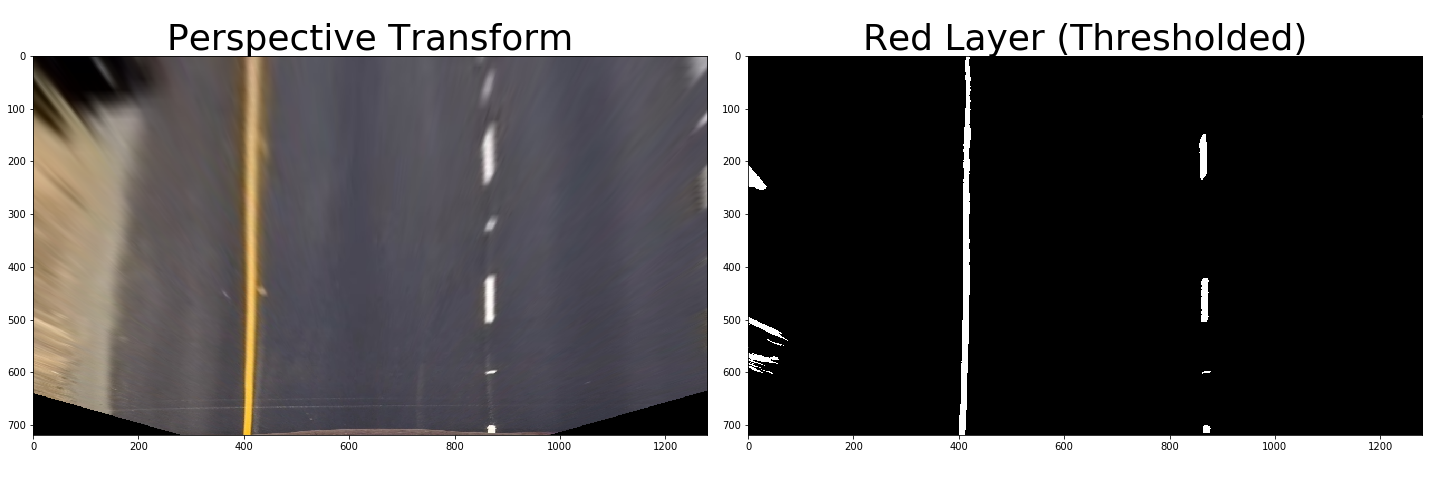
\includegraphics{./output_images/writeup_images/straight_lines1_red.png}

\hypertarget{hls-layers}{%
\paragraph{HLS Layers}\label{hls-layers}}

\begin{center}\rule{0.5\linewidth}{\linethickness}\end{center}

I used the HLS color space to make my \texttt{color\_select()} function
more robust when conditions are not ideal (e.g.~shadows, different road
hue, brightness, etc.). The hue layer is does a good job of finding the
base color independent of brightness which is helpful when shadows are
present. I combined the lightness layer with the hue layer to find
yellow and white values in dark areas. The saturation layer was used to
verify the pixels detected in the low light areas are saturated with a
high enough color value to be confident they are part of the lane line.
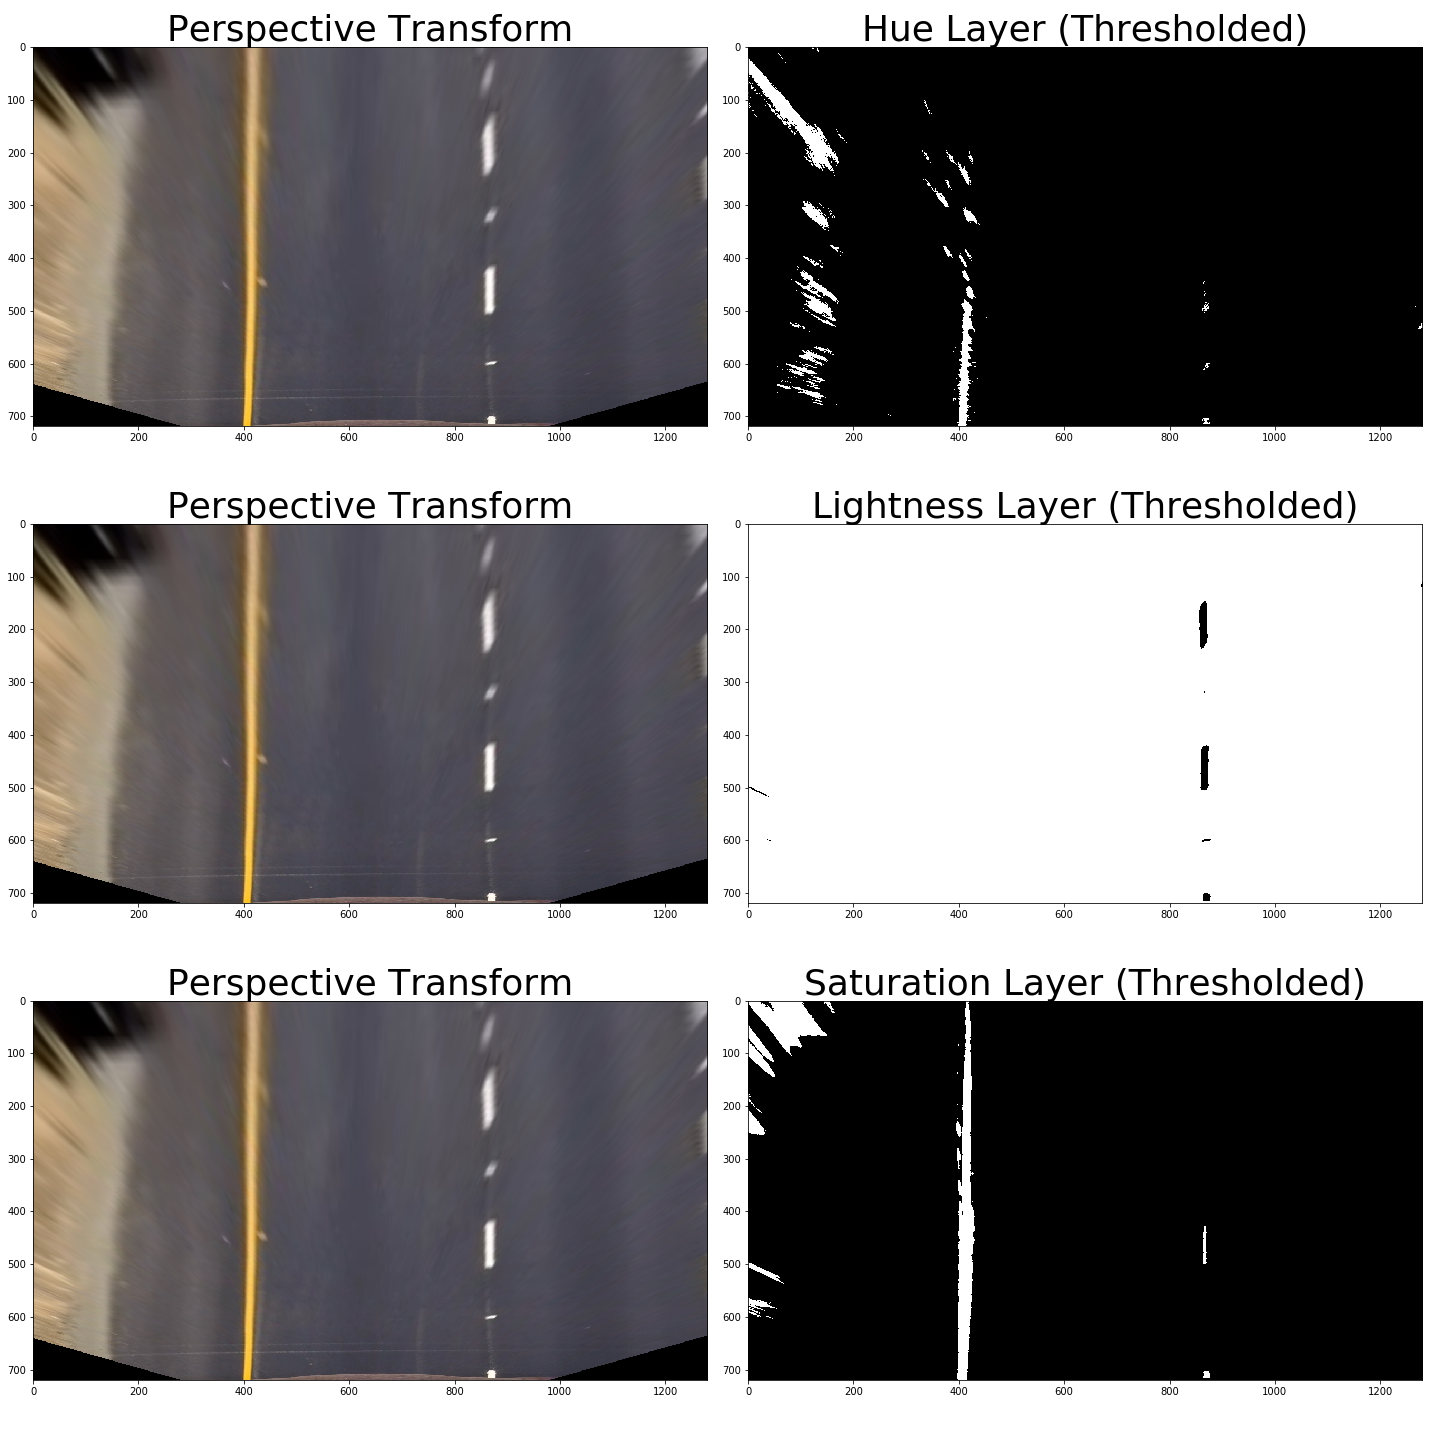
\includegraphics{./output_images/writeup_images/straight_lines1_hls.png}

\hypertarget{combined-color-spaces}{%
\paragraph{Combined Color Spaces}\label{combined-color-spaces}}

\begin{center}\rule{0.5\linewidth}{\linethickness}\end{center}

The results of thresholding the HLS layers and the Red layer are
combined using \texttt{cv2.bitwise\_or()}. An example of the color
selected image is displayed below:\\
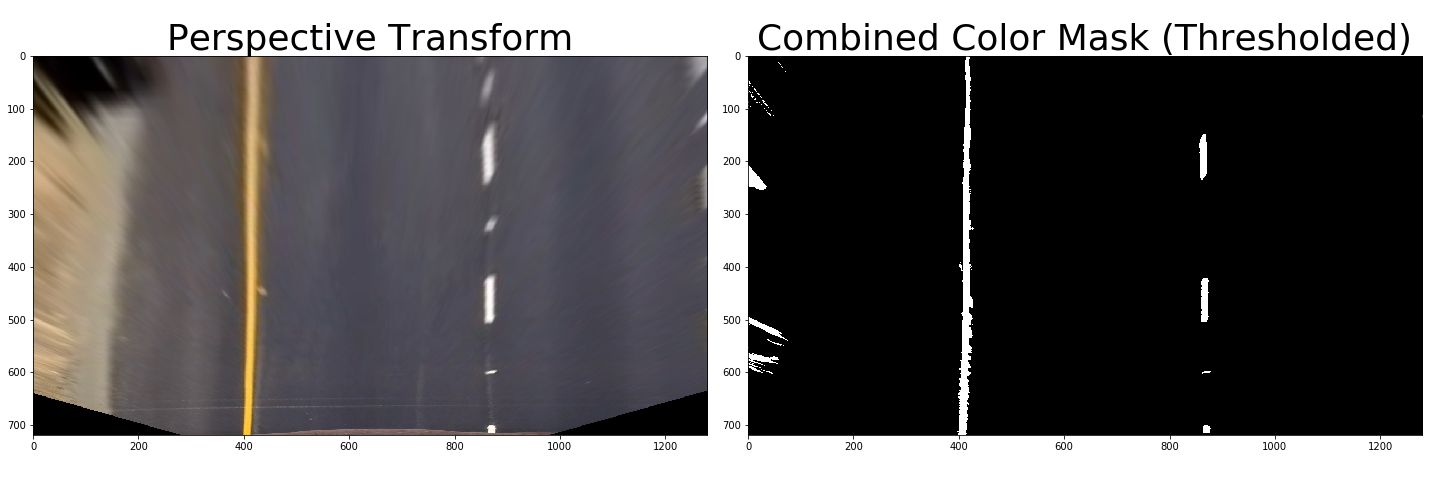
\includegraphics{./output_images/writeup_images/straight_lines1_combined.png}

\hypertarget{gradient-sobel}{%
\paragraph{Gradient (Sobel)}\label{gradient-sobel}}

\begin{center}\rule{0.5\linewidth}{\linethickness}\end{center}

Using the sobel function and a grayscaled copy of the image, I found the
gradient of the x and y dimension and calculated the direction of the
gradient. I thresholded the gradient in the x-dimension to find where
there is a greater change in color intensity value. This is helpful when
finding the side edges of lane lines because the lane lines generally
contrast with the road which will result in a higher gradient value in
the x-dimension. The direction will calculate the direction of the x and
y gradient values. Essentially, I used the direction to be confident
that the detected lane line pixels are more vertical than horizontal.
The direction acts as a mask of the \texttt{color\_select} image and
\texttt{gradx}. Notice the dark areas of the direction image coincide
with the values of the gradient image.

See the code for finding gradients below:

\begin{Shaded}
\begin{Highlighting}[]
\KeywordTok{def}\NormalTok{ sobel(img):}
    \CommentTok{'''}
\CommentTok{    Performs sobel operation to get the gradient in x & y direction.}
\CommentTok{    Thresholds the magnitude direction which is achieved using x & y gradients}
\CommentTok{    Returns images for x-direction gradient and the thresholded magnitude direction. }
\CommentTok{    '''}
\NormalTok{    gray }\OperatorTok{=}\NormalTok{ cv2.cvtColor(img, cv2.COLOR_BGR2GRAY)}
    \CommentTok{# Take the derivative in x & y}
\NormalTok{    sobelx }\OperatorTok{=}\NormalTok{ cv2.Sobel(gray, cv2.CV_64F, }\DecValTok{1}\NormalTok{, }\DecValTok{0}\NormalTok{, ksize}\OperatorTok{=}\DecValTok{3}\NormalTok{)}
\NormalTok{    sobely }\OperatorTok{=}\NormalTok{ cv2.Sobel(gray, cv2.CV_64F, }\DecValTok{0}\NormalTok{, }\DecValTok{1}\NormalTok{, ksize}\OperatorTok{=}\DecValTok{3}\NormalTok{)}
    \CommentTok{# Take the absolute value of the derivative or gradient}
\NormalTok{    abs_sobelx }\OperatorTok{=}\NormalTok{ np.absolute(sobelx)}
\NormalTok{    abs_sobely }\OperatorTok{=}\NormalTok{ np.absolute(sobely)    }
    \CommentTok{# Scale to 8-bit (0 - 255) then convert to type = np.uint8}
\NormalTok{    scaled_sobelx }\OperatorTok{=}\NormalTok{ np.uint8(}\DecValTok{255}\OperatorTok{*}\NormalTok{abs_sobelx}\OperatorTok{/}\NormalTok{np.}\BuiltInTok{max}\NormalTok{(abs_sobelx))}

    \CommentTok{# Create a mask of 1's where the scaled gradient magnitude is within threshold}
\NormalTok{    sobel_thresh }\OperatorTok{=}\NormalTok{ (}\DecValTok{30}\NormalTok{,}\DecValTok{255}\NormalTok{)}
\NormalTok{    gradx }\OperatorTok{=}\NormalTok{ np.zeros_like(scaled_sobelx)}
\NormalTok{    gradx[(scaled_sobelx }\OperatorTok{>=}\NormalTok{ sobel_thresh[}\DecValTok{0}\NormalTok{]) }\OperatorTok{&}\NormalTok{ (scaled_sobelx }\OperatorTok{<=}\NormalTok{ sobel_thresh[}\DecValTok{1}\NormalTok{])] }\OperatorTok{=} \DecValTok{1}
    \CommentTok{# Get the binary image of the thresholded magnitude direction}
\NormalTok{    dir_binary }\OperatorTok{=}\NormalTok{ sobel_mag_dir(abs_sobelx, abs_sobely)}
    \ControlFlowTok{return}\NormalTok{ gradx, dir_binary}

\KeywordTok{def}\NormalTok{ sobel_mag_dir(abs_sobelx, abs_sobely, dir_thresh}\OperatorTok{=}\NormalTok{(}\FloatTok{0.0}\NormalTok{, }\FloatTok{0.3}\NormalTok{)):}
    \CommentTok{''' Returns thesholded binary image of magitude direction from sobel gradients '''}
    \CommentTok{# Calculate absolute direction of gradient}
\NormalTok{    absgraddir }\OperatorTok{=}\NormalTok{ np.arctan2(abs_sobelx, abs_sobely)}
    \CommentTok{# Create binary image of thresholded gradient direction}
\NormalTok{    binary_output }\OperatorTok{=}\NormalTok{ np.zeros_like(absgraddir)}
\NormalTok{    binary_output[(absgraddir }\OperatorTok{>=}\NormalTok{ dir_thresh[}\DecValTok{0}\NormalTok{]) }\OperatorTok{&}\NormalTok{ (absgraddir }\OperatorTok{<=}\NormalTok{ dir_thresh[}\DecValTok{1}\NormalTok{])] }\OperatorTok{=} \DecValTok{1}
    \ControlFlowTok{return}\NormalTok{ binary_output}
\end{Highlighting}
\end{Shaded}

\begin{figure}
\centering
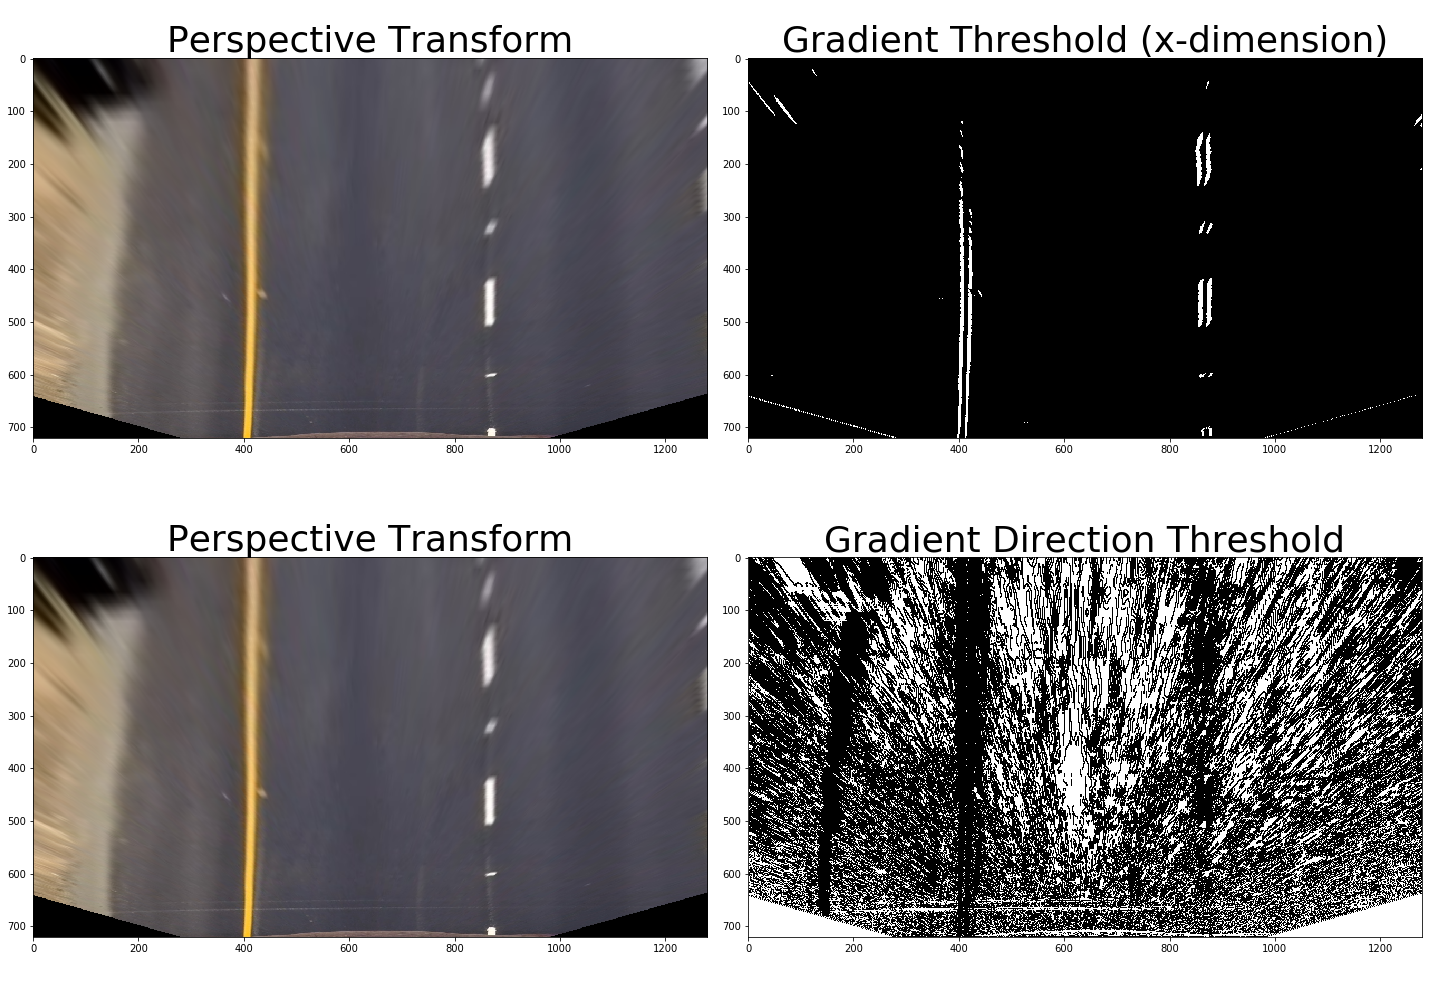
\includegraphics{./output_images/writeup_images/straight_lines1_gradient.png}
\caption{alt\_text}
\end{figure}

\hypertarget{region-of-interest}{%
\paragraph{Region of interest}\label{region-of-interest}}

\begin{center}\rule{0.5\linewidth}{\linethickness}\end{center}

Finally, A region of interest is applied to the result of the color
selected and gradient images to eliminate noise caused by the
surrounding environment (e.g.~grass, adjacent vehicles, etc.)
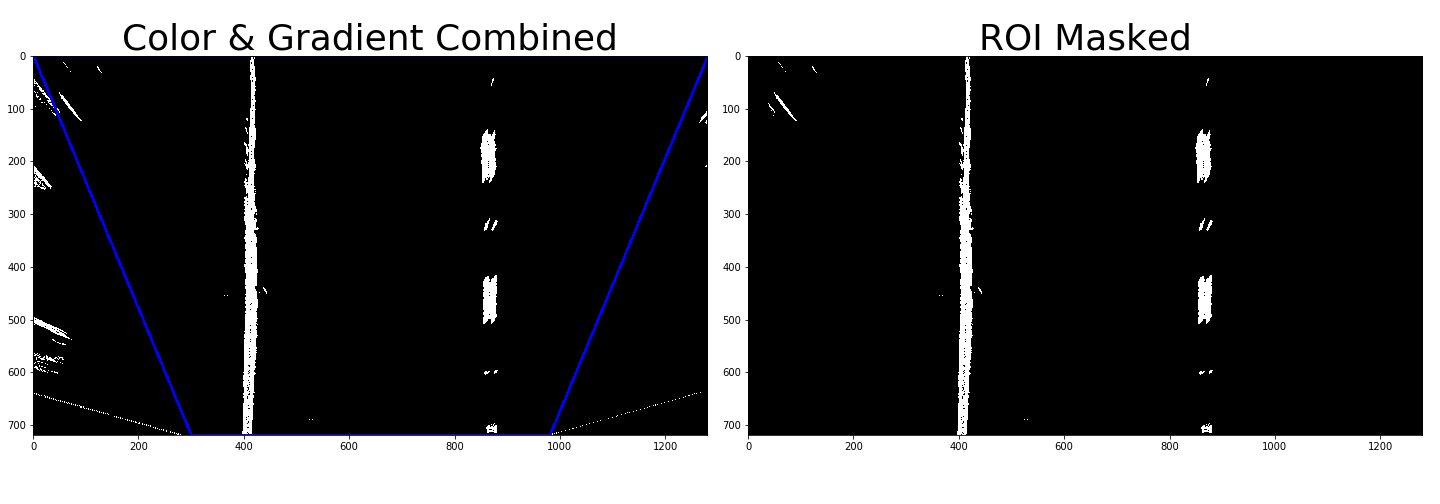
\includegraphics{./output_images/writeup_images/straight_lines1_roi.png}
***

    \hypertarget{have-lane-line-pixels-been-identified-in-the-rectified-image-and-fit-with-a-polynomial}{%
\subsubsection{4. Have lane line pixels been identified in the rectified
image and fit with a
polynomial?}\label{have-lane-line-pixels-been-identified-in-the-rectified-image-and-fit-with-a-polynomial}}

I implemented the moving window to detect the lane line pixels and fit a
polynomial to each line. The window method uses 9 rectangular windows
with a window height equal to the image height divided by 9 and a
defined width to search for lane pixels for each line. To illustrate
this step I will use the example image below:

\begin{figure}
\centering
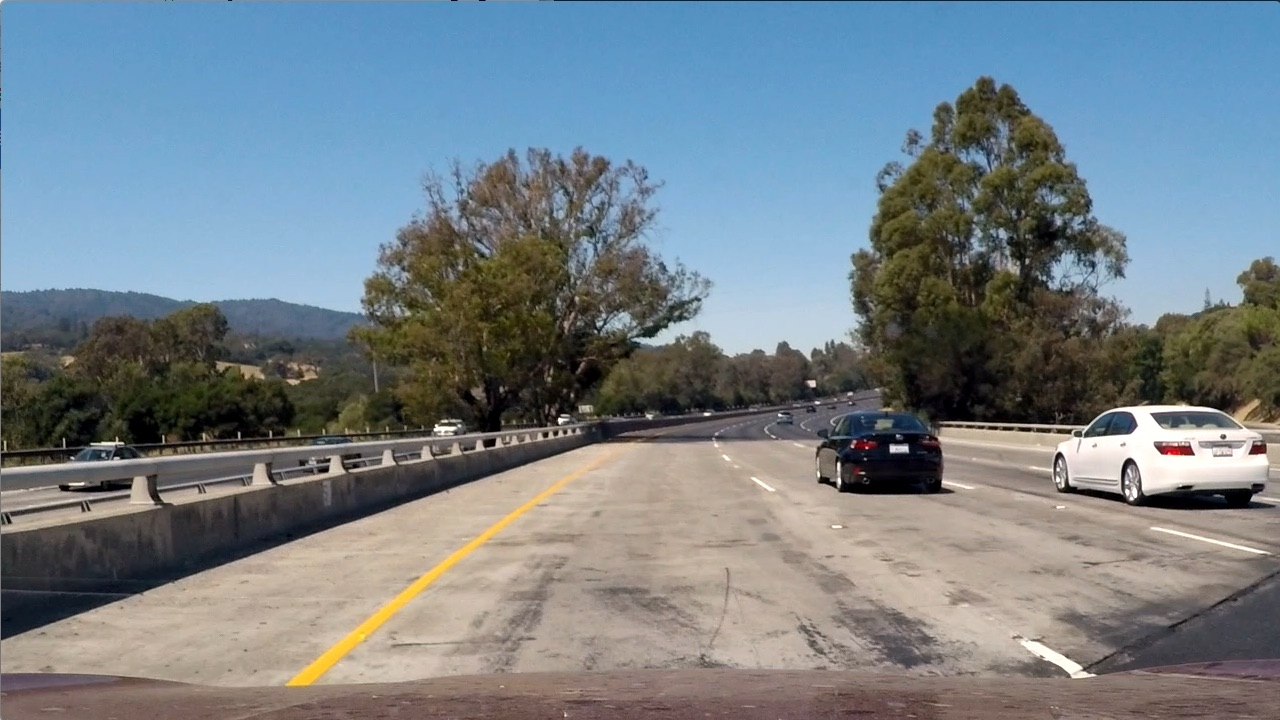
\includegraphics{./test_images/test1.jpg}
\caption{alt\_text}
\end{figure}

\hypertarget{histogram}{%
\paragraph{Histogram}\label{histogram}}

\begin{center}\rule{0.5\linewidth}{\linethickness}\end{center}

The position of the first rectangle is found by using a histogram on the
bottom half of the image to identify the x-value that contains the most
white pixels for the left and right lane line. In the example histogram
below, the x-values for each value would be Left: \textasciitilde{}420
Right: \textasciitilde{}940
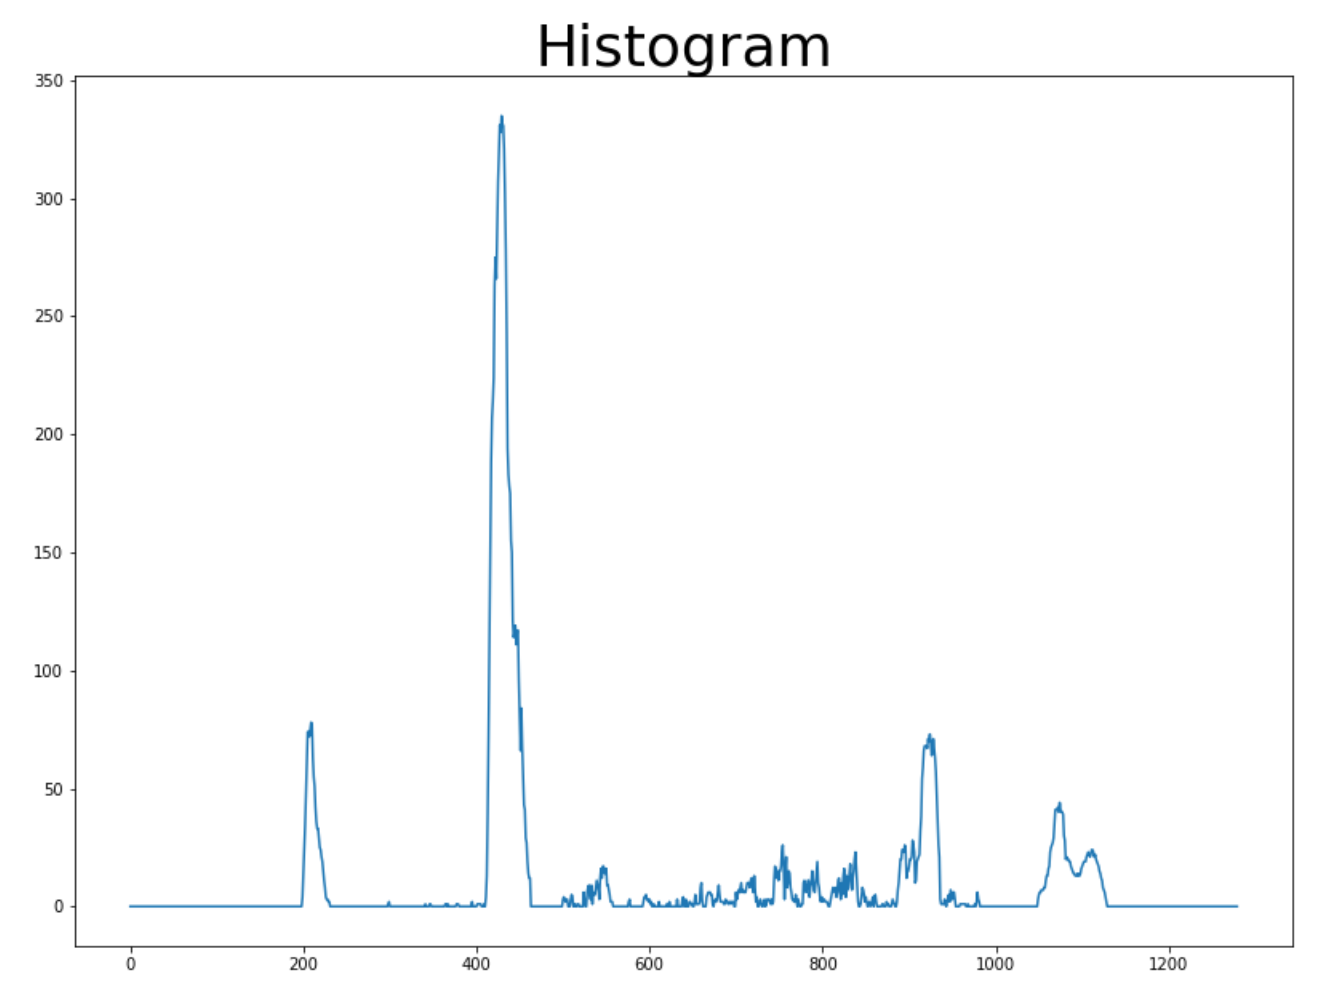
\includegraphics{./output_images/writeup_images/test1_histogram.png}

\hypertarget{window-search-and-polynomial}{%
\paragraph{Window Search and
Polynomial}\label{window-search-and-polynomial}}

\begin{center}\rule{0.5\linewidth}{\linethickness}\end{center}

The first windows are centered at the bottom of the image on the
x-values found in the historam search and searches for lane pixels. If
the amount of pixels found in the rectangle is greater than
\texttt{minpix}, the window is re-centered at the average x-value of the
detected pixels coordinates. This continues until all windows have been
searched. A polynomial is fitted to the detected lane line pixels using
\texttt{np.polyfit()}. See the example result below:
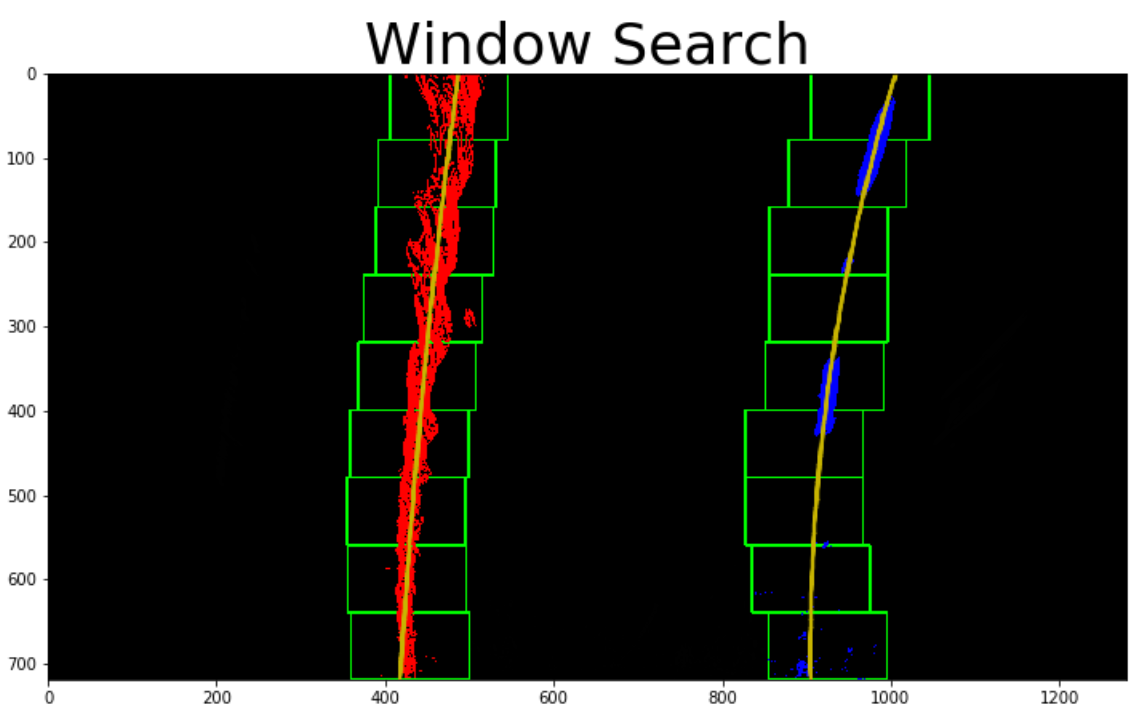
\includegraphics{./output_images/writeup_images/test1_window.png}

    \hypertarget{having-identified-the-lane-lines-has-the-radius-of-curvature-of-the-road-been-estimated-and-the-position-of-the-vehicle-with-respect-to-center-in-the-lane}{%
\subsubsection{5. Having identified the lane lines, has the radius of
curvature of the road been estimated? And the position of the vehicle
with respect to center in the
lane?}\label{having-identified-the-lane-lines-has-the-radius-of-curvature-of-the-road-been-estimated-and-the-position-of-the-vehicle-with-respect-to-center-in-the-lane}}

\hypertarget{radius-of-curvature}{%
\paragraph{Radius of Curvature}\label{radius-of-curvature}}

The radius of curvature estimation was identified by calculating the
radius of each line individualy using the radius equation and then
taking the average of two radii. To report this value in meters, I first
assigned a metric value per pixel in each dimension. For the
y-dimension, I used 30 meters as an estimate of the maximum distance
from the vehicle that the perspective transform rectifies. For the
x-dimension, I divide the standard lane width of 3.7 meters by the
difference between the x-intercepts of each lane line polynomial.

\begin{Shaded}
\begin{Highlighting}[]
\KeywordTok{def}\NormalTok{ curvature_radius_real(y_vals, left, right):}
    \CommentTok{''' Calculates current radius of curvature in meters '''}
    \CommentTok{# Assign metric value to pixels in each dimension}
\NormalTok{    ym_per_pix }\OperatorTok{=} \DecValTok{30}\OperatorTok{/}\DecValTok{720}  \CommentTok{# meters per pixel in y dimension}
\NormalTok{    xm_per_pix }\OperatorTok{=} \FloatTok{3.7}\OperatorTok{/}\NormalTok{(right.best_fit[}\OperatorTok{-}\DecValTok{1}\NormalTok{] }\OperatorTok{-}\NormalTok{ left.best_fit[}\OperatorTok{-}\DecValTok{1}\NormalTok{]) }\CommentTok{# meters per pixel in x dimension}
    
\NormalTok{    y_eval }\OperatorTok{=}\NormalTok{ np.}\BuiltInTok{max}\NormalTok{(y_vals)}
    
    \CommentTok{# Convert best fit polynomial to real world values}
\NormalTok{    left_fit_cr }\OperatorTok{=}\NormalTok{ np.polyfit(y_vals}\OperatorTok{*}\NormalTok{ym_per_pix, left.bestx}\OperatorTok{*}\NormalTok{xm_per_pix, }\DecValTok{2}\NormalTok{)}
\NormalTok{    right_fit_cr }\OperatorTok{=}\NormalTok{ np.polyfit(y_vals}\OperatorTok{*}\NormalTok{ym_per_pix, right.bestx}\OperatorTok{*}\NormalTok{xm_per_pix, }\DecValTok{2}\NormalTok{)}
    
    \CommentTok{# Calculate radius of curvature}
\NormalTok{    left.radius_of_curvature }\OperatorTok{=}\NormalTok{ ((}\DecValTok{1} \OperatorTok{+}\NormalTok{ (}\DecValTok{2}\OperatorTok{*}\NormalTok{left_fit_cr[}\DecValTok{0}\NormalTok{]}\OperatorTok{*}\NormalTok{y_eval}\OperatorTok{*}\NormalTok{ym_per_pix }\OperatorTok{+}\NormalTok{ left_fit_cr[}\DecValTok{1}\NormalTok{])}\OperatorTok{**}\DecValTok{2}\NormalTok{)}\OperatorTok{**}\FloatTok{1.5}\NormalTok{) }\OperatorTok{/}\NormalTok{ np.absolute(}\DecValTok{2}\OperatorTok{*}\NormalTok{left_fit_cr[}\DecValTok{0}\NormalTok{])}
\NormalTok{    right.radius_of_curvature }\OperatorTok{=}\NormalTok{ ((}\DecValTok{1} \OperatorTok{+}\NormalTok{ (}\DecValTok{2}\OperatorTok{*}\NormalTok{right_fit_cr[}\DecValTok{0}\NormalTok{]}\OperatorTok{*}\NormalTok{y_eval}\OperatorTok{*}\NormalTok{ym_per_pix }\OperatorTok{+}\NormalTok{ right_fit_cr[}\DecValTok{1}\NormalTok{])}\OperatorTok{**}\DecValTok{2}\NormalTok{)}\OperatorTok{**}\FloatTok{1.5}\NormalTok{) }\OperatorTok{/}\NormalTok{ np.absolute(}\DecValTok{2}\OperatorTok{*}\NormalTok{right_fit_cr[}\DecValTok{0}\NormalTok{])}
\end{Highlighting}
\end{Shaded}

\hypertarget{vehicle-position}{%
\paragraph{Vehicle Position}\label{vehicle-position}}

The vehicle position is calculated by first finding the difference
between the x-intercept of the lane line and the center of the image,
which is assumed to be the center of the vehicle. Then, I add the
differences together. This value represents the vehicle position
relative to the lane center. If this value is negative, the vehicle is
left of center. If positive, the vehicle is right of the lane center.

\begin{Shaded}
\begin{Highlighting}[]
\KeywordTok{def}\NormalTok{ vehicle_offset(img, left, right):}
    \CommentTok{''' Calculates difference between vehicle center and lane center '''}
\NormalTok{    vehicle_center }\OperatorTok{=}\NormalTok{ img.shape[}\DecValTok{1}\NormalTok{] }\OperatorTok{//} \DecValTok{2}  \CommentTok{# center of vehicle is center of image}
\NormalTok{    xm_per_pix }\OperatorTok{=} \FloatTok{3.7} \OperatorTok{/}\NormalTok{ (right.bestx[}\OperatorTok{-}\DecValTok{1}\NormalTok{] }\OperatorTok{-}\NormalTok{ left.bestx[}\OperatorTok{-}\DecValTok{1}\NormalTok{])  }\CommentTok{# x-values of line nearest the vehicle}
    \CommentTok{# Calculate x-value of lane center}
\NormalTok{    left.line_base_pos }\OperatorTok{=}\NormalTok{ left.bestx[}\OperatorTok{-}\DecValTok{1}\NormalTok{] }\OperatorTok{-}\NormalTok{ vehicle_center    }\CommentTok{# expects negative value}
\NormalTok{    right.line_base_pos }\OperatorTok{=}\NormalTok{ right.bestx[}\OperatorTok{-}\DecValTok{1}\NormalTok{] }\OperatorTok{-}\NormalTok{ vehicle_center  }\CommentTok{#expects positive value}
\NormalTok{    vehicle_offset }\OperatorTok{=}\NormalTok{ left.line_base_pos }\OperatorTok{+}\NormalTok{ right.line_base_pos}
    \ControlFlowTok{return}\NormalTok{ vehicle_offset}\OperatorTok{*}\NormalTok{xm_per_pix}
\end{Highlighting}
\end{Shaded}

An example of a processed image with the radius and vehicle position is
shown below:
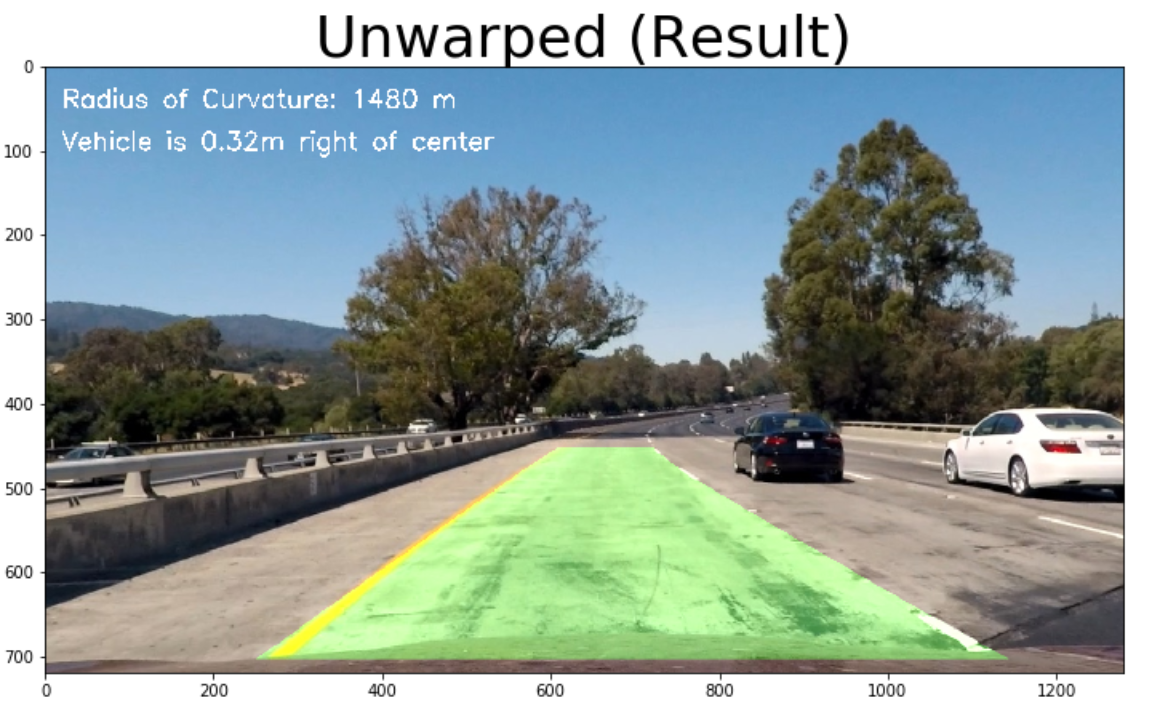
\includegraphics{./output_images/writeup_images/test1_rad.png} ***

    \hypertarget{pipeline-video}{%
\subsection{Pipeline (video)}\label{pipeline-video}}

\begin{center}\rule{0.5\linewidth}{\linethickness}\end{center}

\hypertarget{does-the-pipeline-established-with-the-test-images-work-to-process-the-video-has-some-kind-of-search-method-been-implemented-to-discover-the-position-of-the-lines-in-the-first-images-in-the-video-stream-has-some-form-of-tracking-of-the-position-of-the-lane-lines-been-implemented}{%
\subsubsection{Does the pipeline established with the test images work
to process the video? Has some kind of search method been implemented to
discover the position of the lines in the first images in the video
stream? Has some form of tracking of the position of the lane lines been
implemented?}\label{does-the-pipeline-established-with-the-test-images-work-to-process-the-video-has-some-kind-of-search-method-been-implemented-to-discover-the-position-of-the-lines-in-the-first-images-in-the-video-stream-has-some-form-of-tracking-of-the-position-of-the-lane-lines-been-implemented}}

The same pipeline that is used to process the test images is used to
process the video. However, when processing a video, I use a more
effiecient method of finding the lane pixels once a lane has been
successfully detected. This method will search arround the previous
polynomial to detect the new lane pixels which will reject outliers.
This will improve the robustness of detecting the lane line from frame
to frame as the position of lane lines should have little variation
between frames. (See in code comments in \texttt{fit\_polynomial} and
\texttt{search\_around\_poly} for more detailed explanation). See the
result of the processed video in the output file
\texttt{project\_video\_output.mp4}.

A class \texttt{Line()} is used to keep track of each lane line and
allows for a weighted average calculation of previous lines. Code shown
below:

\begin{Shaded}
\begin{Highlighting}[]
\CommentTok{##################### CREATE 'Line()' CLASS ######################}
\KeywordTok{class}\NormalTok{ Line:}
    \KeywordTok{def} \FunctionTok{__init__}\NormalTok{(}\VariableTok{self}\NormalTok{):}
        \CommentTok{# was the line detected in the last iteration?}
        \VariableTok{self}\NormalTok{.detected }\OperatorTok{=} \VariableTok{False}  
        \CommentTok{# x values of the last n fits of the line}
        \VariableTok{self}\NormalTok{.recent_xfitted }\OperatorTok{=}\NormalTok{ deque() }
        \CommentTok{#average x values of the fitted line over the last n iterations}
        \VariableTok{self}\NormalTok{.bestx }\OperatorTok{=} \VariableTok{None}    
        \CommentTok{#polynomial coefficients averaged over the last n iterations}
        \VariableTok{self}\NormalTok{.best_fit }\OperatorTok{=} \VariableTok{None}  
        \CommentTok{#polynomial coefficients for the most recent fit}
        \VariableTok{self}\NormalTok{.current_fit }\OperatorTok{=}\NormalTok{ np.array([])  }
        \CommentTok{#radius of curvature of the line in some units}
        \VariableTok{self}\NormalTok{.radius_of_curvature }\OperatorTok{=} \VariableTok{None} 
        \CommentTok{#distance in meters of vehicle center from the line}
        \VariableTok{self}\NormalTok{.line_base_pos }\OperatorTok{=} \VariableTok{None} 
        \CommentTok{#difference in fit coefficients between last and new fits}
        \VariableTok{self}\NormalTok{.diffs }\OperatorTok{=}\NormalTok{ np.array([}\DecValTok{0}\NormalTok{,}\DecValTok{0}\NormalTok{,}\DecValTok{0}\NormalTok{], dtype}\OperatorTok{=}\StringTok{'float'}\NormalTok{) }
        \CommentTok{#x values for detected line pixels}
        \VariableTok{self}\NormalTok{.allx }\OperatorTok{=} \VariableTok{None}
        \CommentTok{#y values for detected line pixels}
        \VariableTok{self}\NormalTok{.ally }\OperatorTok{=} \VariableTok{None}  
\end{Highlighting}
\end{Shaded}

\begin{center}\rule{0.5\linewidth}{\linethickness}\end{center}

\hypertarget{sanity-checks}{%
\paragraph{Sanity Checks}\label{sanity-checks}}

I used some sanity checks to find the best fit for the lane line. After
the lane pixels have been detected, a polynomial has been found, and the
fitted x-values have been found I implement the following sanity checks:
* check for the currently (most recent polynomial) poly-fitted
coefficients. This ensures a line is currently fitted to the line. If
none present, set the detected polynomial to the `current\_fit'. * check
the x-intercepts (x-values at bottom of image) of the new calculated fit
against the current fit. * check the x-value at the top of the
polynomial of the best x-values of the currently fitted polynomial
against the x-fitted values of the new detected line.

These checks will ensure that line fitted by the detected line pixels is
similar to the previous lane line. I provide a +/-50 pixel window for
the x-intercept and +/-60 pixels for the top x-value. I give an extra
+/-10 pixels for the top because this is area where the camera will
first see any curves, which can make cause the end of the lane line
shift more quickly between frames compared to the x-intercept at the
bottom of the image.

The following snippet of code are the sanity inside
\texttt{fit\_polinomial}

\begin{Shaded}
\begin{Highlighting}[]
\CommentTok{# Sanity checks for x-intercepts and x values }
\ControlFlowTok{if}\NormalTok{ ((}\BuiltInTok{len}\NormalTok{(left.current_fit) }\OperatorTok{>} \DecValTok{1}\NormalTok{) }\OperatorTok{&}\NormalTok{ (}\BuiltInTok{len}\NormalTok{(right.current_fit) }\OperatorTok{>} \DecValTok{1}\NormalTok{)):}
    \CommentTok{# Find difference between the best }
\NormalTok{    left.diffs }\OperatorTok{=}\NormalTok{ np.}\BuiltInTok{abs}\NormalTok{(left_fit }\OperatorTok{-}\NormalTok{ left.current_fit)}
\NormalTok{    right.diffs }\OperatorTok{=}\NormalTok{ np.}\BuiltInTok{abs}\NormalTok{(right_fit }\OperatorTok{-}\NormalTok{ right.current_fit)}
\NormalTok{    left_x_diff }\OperatorTok{=}\NormalTok{ np.}\BuiltInTok{abs}\NormalTok{(left_fitx[}\DecValTok{0}\NormalTok{] }\OperatorTok{-}\NormalTok{ left.bestx[}\DecValTok{0}\NormalTok{])}
\NormalTok{    right_x_diff }\OperatorTok{=}\NormalTok{ np.}\BuiltInTok{abs}\NormalTok{(right_fitx[}\DecValTok{0}\NormalTok{] }\OperatorTok{-}\NormalTok{ right.bestx[}\DecValTok{0}\NormalTok{])}

    \CommentTok{# Sanity checks}
    \CommentTok{# Left line - check if similar to current line}
    \ControlFlowTok{if}\NormalTok{ ((left.diffs[}\DecValTok{2}\NormalTok{] }\OperatorTok{<} \DecValTok{50}\NormalTok{) }\OperatorTok{&}\NormalTok{ (left_x_diff }\OperatorTok{<} \DecValTok{60}\NormalTok{)):}
\NormalTok{        left.detected }\OperatorTok{=} \VariableTok{True}
\NormalTok{        left.current_fit }\OperatorTok{=}\NormalTok{ left_fit}
\NormalTok{        left.bestx }\OperatorTok{=}\NormalTok{ weighted_average(left, left_fitx)}
    \CommentTok{# New line is not similar to current, try window search for next frame }
    \ControlFlowTok{else}\NormalTok{:}
\NormalTok{        left.detected }\OperatorTok{=} \VariableTok{False}
\NormalTok{        left.current_fit }\OperatorTok{=}\NormalTok{ []}
\NormalTok{        left.bestx }\OperatorTok{=}\NormalTok{ weighted_average(left, left_fitx)}
\NormalTok{        left.recent_xfitted.clear}

    \CommentTok{# Right Line - check if similar to current line}
    \ControlFlowTok{if}\NormalTok{ ((right.diffs[}\DecValTok{2}\NormalTok{] }\OperatorTok{<} \DecValTok{50}\NormalTok{) }\OperatorTok{&}\NormalTok{ (right_x_diff }\OperatorTok{<} \DecValTok{60}\NormalTok{)):}
\NormalTok{        right.detected }\OperatorTok{=} \VariableTok{True}
\NormalTok{        right.current_fit }\OperatorTok{=}\NormalTok{ right_fit}
\NormalTok{        right.bestx }\OperatorTok{=}\NormalTok{ weighted_average(right, right_fitx)}
    \CommentTok{# New line is not similar to current, try window search for next frame }
    \ControlFlowTok{else}\NormalTok{:}
\NormalTok{        right.detected }\OperatorTok{=} \VariableTok{False}
\NormalTok{        right.current_fit }\OperatorTok{=}\NormalTok{ []}
\NormalTok{        right.bestx }\OperatorTok{=}\NormalTok{ weighted_average(right, right_fitx)}
\NormalTok{        right.recent_xfitted.clear}

\CommentTok{# If no current_fit, set it as the new fit (e.g. first frame, error)         }
\ControlFlowTok{else}\NormalTok{:}
\NormalTok{    left.detected }\OperatorTok{=} \VariableTok{True}
\NormalTok{    right.detected }\OperatorTok{=} \VariableTok{True}
\NormalTok{    left.current_fit }\OperatorTok{=}\NormalTok{ left_fit}
\NormalTok{    right.current_fit }\OperatorTok{=}\NormalTok{ right_fit}
    \CommentTok{# Set bestx as new x-fitted values if empty, otherwise clear queue }
    \ControlFlowTok{if}\NormalTok{ left.bestx }\OperatorTok{==} \VariableTok{None}\NormalTok{:}
\NormalTok{        left.bestx }\OperatorTok{=}\NormalTok{ left_fitx}
    \ControlFlowTok{else}\NormalTok{:}
\NormalTok{        left.recent_xfitted.clear}

    \ControlFlowTok{if}\NormalTok{ right.bestx }\OperatorTok{==} \VariableTok{None}\NormalTok{:}
\NormalTok{        right.bestx }\OperatorTok{=}\NormalTok{ right_fitx}
    \ControlFlowTok{else}\NormalTok{:}
\NormalTok{        right.recent_xfitted.clear}
\end{Highlighting}
\end{Shaded}

\hypertarget{determine-best-fit}{%
\paragraph{Determine Best Fit}\label{determine-best-fit}}

After multiple lane lines have been detected, I determine the best fit
for the line by applying a weighted average to the previous 7
successfully detected lane lines. If a lane line is not detected, the
weighted average will decrease the queue of x-fitted values starting
with the oldest set. This would continue for multiple frames with missed
lane lines until it is empty. If the queue empties, the code will revert
back to the window serach function for detecting lane lines and build
the queue back up. The \texttt{weighted\_average()} function is shown
below:

\begin{Shaded}
\begin{Highlighting}[]
\KeywordTok{def}\NormalTok{ weighted_average(h, fitx, n}\OperatorTok{=}\DecValTok{7}\NormalTok{):}
    \CommentTok{""" }
\CommentTok{    Applies a weighted average to last 'n' x-fitted values.}
\CommentTok{    }
\CommentTok{    h: handle of class object}
\CommentTok{    """}
\NormalTok{    weights}\OperatorTok{=}\NormalTok{[}\DecValTok{1}\NormalTok{,}\DecValTok{1}\NormalTok{,}\DecValTok{2}\NormalTok{,}\DecValTok{3}\NormalTok{,}\DecValTok{5}\NormalTok{,}\DecValTok{8}\NormalTok{,}\DecValTok{13}\NormalTok{]}\CommentTok{#,21,34,55]}
\NormalTok{    run_len }\OperatorTok{=} \BuiltInTok{len}\NormalTok{(h.recent_xfitted)  }\CommentTok{# get current length of queue}

    \CommentTok{# Maintaining running window |f0,f1,f2,...,fn| of previous n x-values}
    \ControlFlowTok{if}\NormalTok{ fitx }\KeywordTok{is} \KeywordTok{not} \VariableTok{None}\NormalTok{:}
        \ControlFlowTok{if}\NormalTok{ run_len }\OperatorTok{==}\NormalTok{ n:  }\CommentTok{# queue is full}
\NormalTok{            h.recent_xfitted.popleft()  }\CommentTok{# [f0<--,|f1,f2,...,fn|,fn+1]}
        \ControlFlowTok{else}\NormalTok{:             }\CommentTok{# queue not full}
\NormalTok{            run_len }\OperatorTok{+=} \DecValTok{1}  \CommentTok{# add 1 to length}
\NormalTok{        h.recent_xfitted.append(fitx)  }\CommentTok{# [f0,|f1,f2,...,fn<--|,fn+1]}
    \ControlFlowTok{else}\NormalTok{:  }\CommentTok{# reduce queue if no x-fitted values are found}
        \ControlFlowTok{if} \BuiltInTok{len}\NormalTok{(h.recent_xfitted) }\OperatorTok{>} \DecValTok{0}\NormalTok{:}
\NormalTok{            h.recent_xfitted.popleft()}
\NormalTok{            run_len }\OperatorTok{-=} \DecValTok{1}

    \CommentTok{# Compute weighted average}
    \ControlFlowTok{if} \BuiltInTok{len}\NormalTok{(h.recent_xfitted) }\OperatorTok{>} \DecValTok{0}\NormalTok{:}
\NormalTok{        h.bestx }\OperatorTok{=}\NormalTok{ np.average(h.recent_xfitted, axis}\OperatorTok{=}\DecValTok{0}\NormalTok{, weights}\OperatorTok{=}\NormalTok{weights[:run_len])}
    \ControlFlowTok{return}\NormalTok{ h.bestx}
\end{Highlighting}
\end{Shaded}

\begin{center}\rule{0.5\linewidth}{\linethickness}\end{center}

Here is a link to my \href{./project_video_output.mp4}{Processed Video}
***

    \hypertarget{discussion}{%
\subsection{Discussion}\label{discussion}}

In this section, I will explain my pipeline and any improvements I would
make if I pursued this project further.

\hypertarget{pipeline-explanation}{%
\subsubsection{Pipeline Explanation}\label{pipeline-explanation}}

\begin{center}\rule{0.5\linewidth}{\linethickness}\end{center}

NOTE: Before the pipeline is used, a Line() instance must be created for
each lane line. 1. Create copy of input image 2. Undistort image using
the calibration data obtained from \texttt{camera\_calibration.ipynb}
code 3. Get a ``birds-eye'' view of the lane * I do this before I
perform color selection and gradient functions because the transformed
will have nearly vertical lines which is an advantage when filtering the
direction gradient. Also, there will be less noise caused by the scene
surrounding the region being transformed, effectively making the
detection of colors and gradients more robust. 4. Use HLS color spacce
and Red layer of the image to find lane line pixels. * HLS color space
improves robustness of Red layer thresholding to ensure the pixel values
represent yellow or white values. * HLS also improves the ability to
detect lane lines with varying pavement color and when shadows are
present. 5. Gradients are used to find where difference in intensity
values from one pixel to the next is significant. * This allows me to
find the edges of the lane line because the contrast between the lane
line and the pavement color is generally significant. * I used the
gradient magnitude direction as a mask to filter pixels that might not
be be part of the line. The direction will find pixels that are not
\textsubscript{mostly} vertical. This will result in dark (filled with
`0') areas where the lane lines should be which will be and-ed with the
combined image of color\_select and the gradient of x-dimension. 6. Find
lane pixels * If no previous lines detected, use window search * If
previous lines detected, search around previous polynomial * Get
polynomial of lane line pixels and the x values of polynomial * If there
is a previously detected line, use sanity checks to determine the best
fit using a weighted average of previous 6 frames and the new x-fitted
values. If the line does not pass the sanity checks, include it in the
weighted average but use the window search for the next frame and clear
the queue of previous x-fitted values. This will refresh the weighted
average to focus on new detections which may have been caused by a sharp
curve or a change in road pavement. * If no lines were detected at all,
the new fit is set as the previous best fit and the queue is cleared. 7.
Radius of curvature in meters * Set a metric value per pixel in each
dimension using standard road width and the difference of the
x-incercept of the detected lane line polynomial. * Fit metric-scaled
polynomial * Use radius formula to find the radius in meters. * Average
the two radius values to get a decent estimate of overal curve. 8. Find
vehicle position relative to the lane center in meters * Find difference
from x-intercept of each line to the center * Add diferences together
and scale result using x-dimension scale factor * If result is negative,
vehicle is left of lane center. If result is positive, vehicle is right
of center. 9. Unwarp image using `Minv' to display detected lane on the
original image 10. Write radius of curvature and vehicle position on
unwarped image

\hypertarget{potential-improvements}{%
\subsubsection{Potential Improvements}\label{potential-improvements}}

\begin{center}\rule{0.5\linewidth}{\linethickness}\end{center}

\begin{itemize}
\tightlist
\item
  Implement more dynamic transform region for ``birds-eye'' view for
  more accurate radius of curvature calculation. This will also make the
  processing time slower.
\item
  Implement a solution to help display more accurate lane region when
  vehicle goes over a bump in the road without causing a ripple effect
  on next few detections.
\item
  Use the vehicle center to estimate where to look for the next lane
  line x-intercept.
\item
  Implement a sanity checks to check variation between left and right
  calculations
\end{itemize}


    % Add a bibliography block to the postdoc
    
    
    
    \end{document}
